\documentclass[czech, ba, kiv, he]{fasthesis}
\title{Vytvoření Wordpress pluginu pro vyhledávání předků pro Czech-American TV}
\author{Jan}{Čácha}{}{}
\supervisor{Ing. Martin Dostal, Ph.D.}
\stagworkid{A22B0019P}
\assignment{A22B0019P_zadani.pdf}
\addbibresource{doc.bib} % Odkaz na soubor .bib
\signdate{1}{1}{2025}{V Plzni}
\usepackage{listings}
\usepackage{caption}
\usepackage{float}







% Použití stylu a dalších nastavení
\lstset{style=FASThesisLstStyle, numberblanklines=false, tabsize=5, keywordstyle=\color{red}}

% Přepis literálu pro podporu diakritiky v českém textu
\lstset{literate=%
    {á}{{\'a}}1 {č}{{\v c}}1 {ď}{{\v d}}1 {é}{{\'e}}1 {ě}{{\v e}}1 {í}{{\'i}}1 {ň}{{\v n}}1 
    {ó}{{\'o}}1 {ř}{{\v r}}1 {š}{{\v s}}1 {ť}{{\v t}}1 {ú}{{\'u}}1 {ů}{{\r u}}1 {ý}{{\'y}}1 {ž}{{\v z}}1 
    {Á}{{\'A}}1 {Č}{{\v C}}1 {Ď}{{\v D}}1 {É}{{\'E}}1 {Ě}{{\v E}}1 {Í}{{\'I}}1 {Ň}{{\v N}}1 
    {Ó}{{\'O}}1 {Ř}{{\v R}}1 {Š}{{\v S}}1 {Ť}{{\v T}}1 {Ú}{{\'U}}1 {Ů}{{\r U}}1 {Ý}{{\'Y}}1 {Ž}{{\v Z}}1 
}









\abstract{Tato bakalářská práce se zaměřuje na vývoj WordPress pluginu, který má usnadnit vyhledávání předků pro diváky Czech-American TV. S rostoucím zájmem o genealogii mezi českou diasporou se potřeba efektivních nástrojů pro pátrání po předcích stala zásadní. Projekt začíná analýzou existujících řešení, následovanou shromážděním požadavků od zúčastněných stran, včetně zástupců Czech-American TV. Na základě této analýzy je navržen a implementován nový plugin, který zahrnuje uživatelsky přívětivé funkce pro efektivní vyhledávací možnosti. Plugin je důkladně testován, aby se zajistila jeho spolehlivost a jednoduchost použití. Tato práce přispívá k vylepšení online zážitku pro diváky, kteří se zajímají o zkoumání svého dědictví, a podporuje hlubší spojení s jejich kořeny.}
{This bachelor’s thesis focuses on the development of a WordPress plugin designed to facilitate ancestor searches for viewers of Czech-American TV. With the increasing interest in genealogy among the Czech diaspora, the need for effective tools to trace ancestry has become paramount. The project begins with an analysis of existing solutions, followed by gathering requirements from stakeholders, including representatives from Czech-American TV. Based on this analysis, a new plugin is proposed and implemented, incorporating user-friendly features for efficient search functionalities. The plugin is rigorously tested to ensure reliability and ease of use. This work contributes to enhancing the online experience for viewers interested in exploring their heritage, promoting a deeper connection with their roots.}
\keywords{Bakalářská práce, wordpress, plugin, genealogy}
\acknowledgement{Rád bych vyjádřil upřímné poděkování svému vedoucímu práce, Ing. Martinu Dostalovi, Ph.D., za cenné rady, odborné vedení a trpělivost, kterou mi věnoval během celé práce. Jeho podpora a připomínky mi pomohly posunout projekt na vyšší úroveň.

Dále bych chtěl poděkovat zástupcům Czech-American TV za ochotu spolupracovat a poskytnout cenné podklady a zpětnou vazbu, která mi pomohla lépe pochopit potřeby uživatelů.

Velké díky patří také mé rodině a přátelům za trpělivost, podporu a motivaci během celého procesu psaní této bakalářské práce.

V neposlední řadě děkuji všem, kteří mi jakkoli pomohli, ať už radou, technickou pomocí nebo jen slovy povzbuzení.}
\begin{document}
\frontpages[tm]
\tableofcontents

\chapter{Úvod}

Czech-American TV je nezisková organizace působící ve Spojených státech amerických, která se zaměřuje na podporu, uchovávání a propagaci české kultury, historie a tradic zejména mezi česko-americkou komunitou. Hlavním posláním organizace je budovat most mezi generacemi českých imigrantů a jejich potomky v USA a původními kořeny v České republice a bývalém Československu. Czech-American TV pravidelně tvoří a vysílá televizní pořady, které se věnují české kultuře, významným městům, historickým událostem, památkám a lidovým tradicím.

Vedle televizního vysílání poskytuje organizace také rozsáhlé online zdroje, které napomáhají uživatelům při hledání informací o jejich českých předcích. Mezi tyto zdroje patří genealogické databáze, digitalizované archivní dokumenty, informační weby, interaktivní mapy a vzdělávací programy. Tyto nástroje slouží nejen k objevování vlastních kořenů, ale i k prohlubování znalostí o české historii a tradicích.

V tomto kontextu vzniká tato bakalářská práce, jejímž cílem je vytvořit WordPress plugin, který bude součástí online platformy Czech-American TV a bude dále rozšiřovat možnosti genealogického vyhledávání. Plugin má za úkol zpřístupnit uživatelům různé nástroje sloužící k hledání předků, a to prostřednictvím intuitivního uživatelského rozhraní a propojení s existujícími databázemi a zdroji informací.

Motivace pro realizaci tohoto projektu vychází z rostoucího zájmu o genealogii v digitálním věku. V posledních letech roste počet uživatelů, kteří se zajímají o své předky, rodinnou historii a původ, a to jak v rámci akademického výzkumu, tak i z osobní potřeby. Digitalizace historických záznamů a rozvoj online nástrojů tento trend ještě více podporují.

Česko-americká komunita je přitom skupinou, která často čelí specifickým výzvám — především jazykovým bariérám a roztříštěnosti dostupných zdrojů. Proto je cílem této práce vytvořit centralizovaný, přístupný a uživatelsky přívětivý nástroj, který umožní snadnější vyhledávání informací, propojení s historickými materiály a hlubší porozumění kulturnímu dědictví.

Navrhovaný plugin bude obsahovat moderní prvky interakce, jako jsou dynamické vyhledávání, vizualizace dat nebo propojení s mapovými službami, které zpříjemní a zefektivní uživatelský zážitek. V práci bude kladen důraz jak na technickou implementaci, tak i na využitelnost výsledného řešení v reálném prostředí Czech-American TV.

\chapter{Teoretická část}

\section{Genealogie a její význam v rámci Czech-American TV}  
Genealogie, tedy studium rodokmenů a rodinné historie, má hluboký význam nejen pro historiky, ale i pro jednotlivce, kteří hledají své kořeny a snaží se porozumět svému původu.  

Na platformě Czech-American TV je patrný rostoucí zájem o propojení mezi českou a americkou historií. Tento projekt si klade za cíl vytvořit nástroj integrovaný do této platformy, který usnadní uživatelům vyhledávání jejich předků a pochopení jejich historických souvislostí. Interaktivní nástroj umožní filtrování dat, vizualizaci informací na mapě a možnost překladu mezi češtinou a angličtinou.  


\section{Genealogická mapa České republiky}

Genealogická mapa Czech-American TV České republiky je nástroj umožňující vizualizaci četnosti příjmení v jednotlivých regionech. Tato funkce je užitečná zejména pro zájemce o rodokmeny, kteří chtějí zjistit historické rozložení svého příjmení a případné vazby na určité oblasti.

Princip fungování mapy spočívá v zadání konkrétního příjmení, na základě kterého je provedeno vyhledání jeho výskytu v dostupných databázích. Výsledky jsou poté zobrazovány na interaktivní mapě, kde intenzita zbarvení jednotlivých regionů odpovídá četnosti výskytu daného příjmení.

\begin{figure}[h]  
    \centering  
    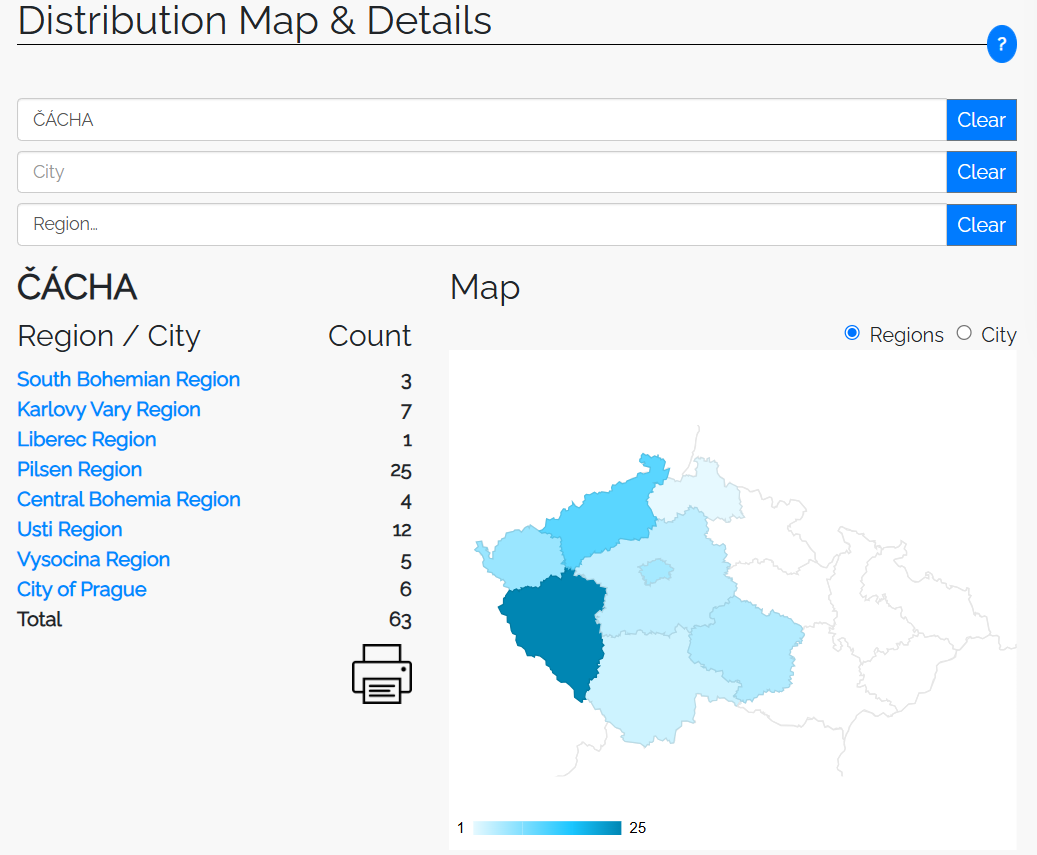
\includegraphics[width=0.8\textwidth]{genealogy_map.png}  
    \caption{Princip fungování mapy}  
\end{figure}

Zdrojová data pro tuto funkcionalitu pocházejí z veřejně dostupných databází obyvatelstva, historických sčítání lidu a dalších genealogických zdrojů. Výzvou při tvorbě této mapy bylo nejen správné zpracování dat, ale také efektivní způsob jejich vizualizace tak, aby bylo možné výsledky snadno interpretovat.

Díky tomuto nástroji mohou uživatelé získat cenné informace o původu svého příjmení a jeho historickém rozšíření v rámci České republiky.




\section{Německo-české názvosloví historických měst}

Historicky měla řada českých měst a obcí své ekvivalenty v německém jazyce, což bylo dáno dlouhodobým soužitím českého a německého obyvatelstva na našem území. Tento dvojjazyčný charakter byl zvláště patrný v pohraničních oblastech a v obdobích, kdy české země byly součástí Rakouska-Uherska.

Mnoho historických dokumentů, map a genealogických záznamů obsahuje názvy měst v jejich německé podobě, což může být matoucí pro dnešní uživatele, kteří hledají české ekvivalenty. Proto vznikla databáze německých a českých názvů, která umožňuje rychlé a snadné přiřazení odpovídajících míst.

Tento nástroj pracuje tak, že uživatel zadá historický německý název města, načež systém vyhledá a zobrazí jeho odpovídající český ekvivalent. Výsledky jsou vizualizovány na mapě, což usnadňuje orientaci v historických geografických údajích.

Tento projekt je cenným přínosem nejen pro genealogické bádání, ale i pro historiky a všechny zájemce o kulturní dědictví českých zemí. [5, 6]


\section{Machine Learning v genealogii}  

Strojové učení představuje moderní technologii, která má v genealogii významný potenciál. Umožňuje analyzovat rozsáhlé soubory historických dat, identifikovat vzory a navrhovat rodinné vztahy na základě pravděpodobnosti. Implementace technik strojového učení v rámci genealogického výzkumu může výrazně zlepšit přesnost a rychlost vyhledávání informací, zejména v případech, kdy se jedná o historicky změněná jména, neúplné záznamy nebo geograficky vzdálené zdroje dat.  

Cílem je vytvořit nástroj, který bude využívat strojové učení k posílení genealogického výzkumu. Součástí tohoto projektu je implementace algoritmu Word2Vec, který bude využit při překladech z češtiny, němčiny a latiny do angličtiny. Word2Vec zde hraje klíčovou roli při rozpoznávání významově příbuzných slov a rozšiřování překladů o relevantní varianty. To zlepší přesnost a srozumitelnost překladů historických dokumentů a umožní uživatelům získat lepší výsledky při vyhledávání genealogických informací.  

\subsection{Word2Vec a jeho využití při překladu}  

Algoritmus Word2Vec je jednou z klíčových metod pro zpracování textových dat v oblasti strojového učení. Tento algoritmus převádí slova do matematických vektorů v mnoharozměrném prostoru, což umožňuje měřit podobnosti mezi nimi pomocí geometrických operací. Model byl poprvé představen v roce 2013 vědci z Google Brain pod vedením Tomáše Mikolova [1] a od té doby se stal základním nástrojem v oblasti zpracování přirozeného jazyka (NLP).  

Word2Vec využívá dva hlavní modely:  

\begin{itemize}  
    \item \textbf{Skip-Gram}: Tento model se snaží předpovědět okolní slova na základě aktuálního slova. Je vhodnější pro malé datové sady, protože je schopný efektivně generalizovat.  
    \item \textbf{CBOW (Continuous Bag of Words)}: Opačný přístup, který se snaží předpovědět aktuální slovo na základě okolních slov. Tento model je často rychlejší než Skip-Gram a lépe funguje s velkými objemy dat.  
\end{itemize}  

Použití Word2Vec v procesu překladu přináší několik výhod:  

\begin{itemize}  
    \item \textbf{Rozšíření překladů o příbuzná slova}: Pokud daný slovník přeloží konkrétní slovo nebo frázi, Word2Vec umožní rozšíření překladu o slova s podobným významem, čímž se zlepší přesnost a přirozenost překladu.  
    \item \textbf{Překonání omezení běžných slovníků}: Historické texty mohou obsahovat méně běžné nebo archaické výrazy, které se nemusí nacházet v dostupných slovnících. Word2Vec pomůže najít jejich modernější nebo příbuzné ekvivalenty.  
    \item \textbf{Podpora kontextového překladu}: Word2Vec umožňuje zohlednit kontext, ve kterém se slovo vyskytuje, což je užitečné při překladu víceznačných termínů.  
\end{itemize}  

\subsection{Matematický model Word2Vec}  

Algoritmus Word2Vec převádí slova na vektory \( \vec{w} \) v n-rozměrném prostoru. Pro optimalizaci těchto vektorů využívá neuronovou síť s jednou skrytou vrstvou, která se učí minimalizovat chybu predikce. Model lze formalizovat následovně:  

\subsubsection{Skip-Gram}  

Skip-Gram model se snaží předpovědět okolní slova \( w_{t+j} \) daného středového slova \( w_t \). Pravděpodobnost výskytu slova \( w_{t+j} \) v kontextu \( w_t \) je definována jako:  

\begin{equation}  
P(w_{t+j} | w_t) = \frac{e^{v'_{w_{t+j}} \cdot v_{w_t}}}{\sum_{w \in V} e^{v'_w \cdot v_{w_t}}}  
\end{equation}  

kde \( v_w \) a \( v'_w \) jsou vektory slov v různých vrstvách modelu a \( V \) je velikost slovníku. Tento výraz odpovídá softmax funkci aplikované na skalární součin vektorů slov.  

\subsubsection{CBOW (Continuous Bag of Words)}  

CBOW model funguje opačně než Skip-Gram – snaží se předpovědět aktuální slovo \( w_t \) na základě jeho kontextu \( C \) (okolních slov). Formálně je pravděpodobnost \( P(w_t | C) \) definována jako:  

\begin{equation}  
P(w_t | C) = \frac{e^{v_{w_t} \cdot \sum_{w_c \in C} v'_{w_c}}}{\sum_{w \in V} e^{v_w \cdot \sum_{w_c \in C} v'_{w_c}}}  
\end{equation}  

Tento vzorec znamená, že pro určení cílového slova \( w_t \) se sčítají vektory jeho okolních slov \( w_c \) a výsledek se transformuje pomocí softmax funkce.  

Vzhledem k výpočetní náročnosti softmaxu se často používají optimalizační techniky jako:  

\begin{itemize}  
    \item \textbf{Negativní vzorkování (Negative Sampling)}: Místo výpočtu pravděpodobnosti pro všechna slova se trénuje model na správná slova a několik negativních příkladů.  
    \item \textbf{Hierarchický softmax}: Nahrazuje klasický softmax binárním stromem, což umožňuje efektivnější výpočty.  
\end{itemize}  

Kromě učení vektorů slov se měří jejich podobnost. Pro měření podobnosti mezi dvěma slovy \( w_1 \) a \( w_2 \) se nejčastěji používá kosinová podobnost:  

\begin{equation}  
\mathrm{cosine\_similarity}(\vec{w}_1, \vec{w}_2) = \frac{\vec{w}_1 \cdot \vec{w}_2}{\|\vec{w}_1\| \cdot \|\vec{w}_2\|}  
\end{equation}  

kde \( \vec{w}_1 \cdot \vec{w}_2 \) je skalární součin a \( \|\vec{w}_1\|, \|\vec{w}_2\| \) jsou velikosti vektorů. Kosinová podobnost nabývá hodnot od -1 do 1, přičemž hodnoty blízké 1 znamenají vysokou podobnost mezi slovy. [4, 3, 2, 13]




\section{Rešerše existujících řešení pro genealogický výzkum}

\subsection{Přehled dostupných genealogických platforem}
V současné době existuje několik významných platforem, které se zaměřují na genealogický výzkum. Mezi nejznámější patří:

\begin{itemize}
    \item \textbf{Ancestry.com} -- Jedna z největších genealogických platforem na světě. Nabízí rozsáhlé databáze historických záznamů, DNA testy a nástroje pro vytváření rodokmenů. Výhodou je obrovské množství dat, nevýhodou vysoká cena předplatného.
    \item \textbf{MyHeritage} -- Platforma zaměřená na propojení rodin po celém světě. Nabízí DNA testy a nástroje pro vizualizaci rodokmenů. Výhodou je uživatelsky přívětivé rozhraní, ale některé funkce jsou dostupné pouze v placené verzi.
    \item \textbf{FamilySearch} -- Bezplatná platforma provozovaná Církví Ježíše Krista Svatých posledních dnů. Obsahuje velké množství digitálních záznamů, vhodná pro začátečníky i pokročilé genealogy. Nevýhodou je menší podpora pro neanglicky mluvící uživatele.
    \item \textbf{Geni.com} -- Platforma zaměřená na spolupráci mezi uživateli při vytváření rodokmenů. Výhodou je sociální aspekt, nevýhodou menší podpora pro samostatný výzkum.
\end{itemize}

\subsection{Srovnání s projektem}
Projekt se od těchto platforem liší v několika klíčových aspektech:

\begin{itemize}
    \item \textbf{Lokalizace} -- Zaměřuje na propojení české a americké historie, což umožňuje hlubší analýzu lokálních dat.
    \item \textbf{Jazyková podpora} -- Překlady mezi češtinou, němčinou, latinou a angličtinou poskytují výhodu při práci s historickými dokumenty.
    \item \textbf{Interaktivní nástroje} -- Genealogická mapa a vizualizace dat usnadňují interpretaci výsledků.
\end{itemize}



\section{Analýza potřeb uživatelů}

Cílovou skupinou projektu jsou genealogičtí nadšenci, historici a rodinní badatelé, kteří se snaží propojit historická data se svými rodokmeny. Klíčovými potřebami těchto uživatelů jsou překlady historických dokumentů, vizuální reprezentace dat, efektivní vyhledávání v databázích a podpora pro neanglicky mluvící uživatele. Projekt tyto potřeby řeší prostřednictvím jazykových nástrojů, genealogických map a využití strojového učení pro vyhledávání v historických datech.

\section{Analýza technologických možností}

\subsection{Výběr Word2Vec a jeho alternativy}

Word2Vec byl vybrán díky své efektivitě při práci s historickými texty, schopnosti rozpoznávat podobnosti mezi slovy a relativně nízké výpočetní náročnosti. Alternativy zahrnují modely jako BERT, GPT, FastText a TF-IDF, z nichž každý má své výhody a nevýhody.

\begin{itemize}
    \item \textbf{BERT} je založen na transformerové architektuře a umožňuje lepší pochopení kontextu, což lze vyjádřit vzorcem:
    \begin{equation}
        h_t = \text{Transformer}(X)
    \end{equation}
    kde \( h_t \) je kontextový vektor slova \( X \), generovaný hlubokými vrstvami modelu. Nevýhodou BERTu je vysoká výpočetní náročnost.

    \item \textbf{GPT} pracuje na principu autoregresivního generování textu, kde pravděpodobnost dalšího slova vychází z Bayesova pravidla:
    \begin{equation}
        P(w_t | w_{1:t-1}) = \frac{P(w_{1:t})}{P(w_{1:t-1})}
    \end{equation}
    Tento přístup je vhodný pro generování textu, ale méně efektivní při hledání podobností mezi historickými výrazy.

    \item \textbf{FastText} rozšiřuje Word2Vec tím, že rozkládá slova na n-gramy, což lze matematicky vyjádřit jako:
    \begin{equation}
        v(w) = \sum_{i=1}^{n} v(g_i)
    \end{equation}
    kde \( g_i \) jsou jednotlivé podslovy slova \( w \). Tento model se lépe hodí pro češtinu díky práci s ohýbanými tvary slov, ale složitější implementace brání jeho využití v projektu.

    \item \textbf{TF-IDF} je jednodušší metoda pro zpracování textu, která se řídí vzorcem:
    \begin{equation}
        \text{TF-IDF}(w) = \text{TF}(w) \times \log \frac{N}{\text{DF}(w)}
    \end{equation}
    kde \( N \) je počet dokumentů a \( \text{DF}(w) \) je počet dokumentů obsahujících slovo \( w \). Tento přístup je rychlý, ale nezachycuje význam slov v kontextu.
\end{itemize}

Vzhledem k tomu, že Word2Vec dokáže efektivně pracovat s historickými dokumenty a má nízkou výpočetní náročnost, byl zvolen jako nejvhodnější řešení.

\section{Analýza datových zdrojů}

Projekt využívá data z historických sčítání lidu, digitálních archivů a veřejných genealogických databází. Kvalita těchto dat je ovlivněna neúplností historických záznamů a regionálními rozdíly v dostupnosti informací. Mezi hlavní výzvy patří normalizace různých formátů, jazykové bariéry u německých a latinských dokumentů a řešení chybějících záznamů, které mohou komplikovat rekonstrukci rodokmenů. [20, 19, 18]

\section{Analýza rizik a omezení}

Technická rizika zahrnují chyby v překladech způsobené omezeními strojového učení a omezenou dostupností historických záznamů. Etická problematika zahrnuje ochranu osobních údajů a citlivost některých historických záznamů. Výsledky projektu jsou také omezeny kvalitou dat a schopností Word2Vec modelu zachytit složitější jazykové kontexty.

\chapter{Analytická část}

Na základě teoretické analýzy byl navržen plugin, který kombinuje výhody WordPressu pro správu obsahu s pokročilými funkcemi strojového učení a geografické vizualizace. Tato kapitola detailně popisuje, jak byly identifikované požadavky převedeny do funkčního řešení. Zaměřuje se na tři klíčové oblasti:
\begin{itemize}
    \item Architekturu pluginu a integraci s WordPress API
    \item Zpracování genealogických dat v Pythonu
    \item Implementaci překladačů a vizualizací
\end{itemize}

\section{Analýza požadavků}

Tato kapitola se zaměřuje na podrobnou analýzu požadavků vyplývajících z potřeb neziskové organizace Czech-American TV, která si klade za cíl zprostředkovat genealogické nástroje členům česko-americké komunity. Výsledkem této analýzy je specifikace funkcionalit, které by měl výsledný WordPress plugin obsahovat, aby naplnil očekávání zadavatele i cílové skupiny uživatelů.

\subsection{Současný stav a motivace ke změně}

Organizace Czech-American TV již v současnosti nabízí na svém webu několik online nástrojů zaměřených na podporu genealogického výzkumu a uchovávání českého kulturního dědictví. Mezi dostupné funkcionality patří například interaktivní genealogická mapa, nástroj pro překlad českých příjmení, informační stránky o změnách jmen po emigraci a instruktážní videa.

Interaktivní mapa využívá geolokační data k vizualizaci výskytu příjmení v jednotlivých oblastech České republiky, což může uživatelům pomoci s lokalizací jejich rodových kořenů. Další funkcí je nástroj pro identifikaci změn v příjmeních, které byly často po příchodu do Spojených států amerických foneticky přizpůsobeny nebo zjednodušeny. Czech-American TV také poskytuje videonávody, které uživatele provádějí základními kroky genealogického výzkumu a využíváním dostupných online nástrojů.

Přestože tyto nástroje tvoří solidní základ, některé aspekty systému by mohly být dále rozvinuty. Například oblast překladů genealogických termínů je omezena pouze na příjmení a chybí podpora běžně používaných latinských nebo německých výrazů z historických matrik. Dále chybí možnost sémantického vyhledávání, které by umožnilo uživatelům najít významově podobné výrazy nebo archaické tvary. Také správa obsahu není plně integrovaná do administračního rozhraní WordPressu, což omezuje možnosti rozšíření a editace dat neprogramátory.

Na základě zpětné vazby od uživatelů a identifikovaných mezer vznikla potřeba doplnit existující řešení o specializovaný plugin pro WordPress, který rozšíří současné funkce o další překladové databáze, interaktivní prvky, moderní vyhledávací algoritmy (např. Word2Vec) a nástroje pro správu obsahu dostupné přímo z administrace webu. Cílem je vytvořit nástroj, který bude přívětivý i pro uživatele bez pokročilých technických znalostí a zároveň nabídne kvalitní podporu pro genealogické bádání.

Zadavatel na základě zkušeností s provozem stávající genealogické sekce a zpětné vazby od uživatelů identifikoval několik oblastí, kde je prostor pro zlepšení a rozšíření funkcionality:

\begin{itemize}
\item Omezené interaktivní prvky – současná genealogická mapa sice zobrazuje výskyt příjmení a některá místa původu, nicméně chybí například propojení s historickými názvy měst, nebo možnost rozšířeného vyhledávání podle různých jazykových podob jmen (např. česká, německá, latinská verze).
\item Nedostatečné pokrytí překladů genealogických termínů – aktuálně dostupné nástroje se zaměřují převážně na příjmení. V historických dokumentech však často figurují i latinské nebo německé výrazy (např. „uxor“, „defunctus“, „geboren“), které mohou být pro běžného uživatele nesrozumitelné.
\item Omezené možnosti správy a úprav dat – stávající systém neumožňuje snadnou aktualizaci překladových databází nebo přidávání nových položek bez přímého zásahu do kódu, což komplikuje udržitelnost projektu z pohledu běžného redaktora.
\item Absence sémantického vyhledávání – současný systém nenabízí funkci, která by uživateli pomohla nalézt významově podobné výrazy, archaické formy slov nebo termíny s podobným významem.
\end{itemize}

Z těchto důvodů vznikl návrh na vývoj specializovaného pluginu pro redakční systém WordPress, který rozšíří stávající možnosti Czech-American TV o nové interaktivní nástroje pro genealogické vyhledávání, správu překladových databází a sémantické vyhledávání. Plugin bude navržen tak, aby byl snadno použitelný jak pro koncové uživatele, tak pro administrátory bez nutnosti technických znalostí.

\subsection{Cílová skupina a specifika}

Uživatelskou základnu tvoří především američtí potomci českých imigrantů, kteří často neumí česky, případně mají omezené historické znalosti o českých reáliích. Z tohoto důvodu je nutné, aby byl systém jazykově přívětivý a intuitivní. Důraz musí být kladen na přehlednost a snadnou použitelnost, přičemž plugin by měl fungovat jako prostředník mezi uživatelem a komplexními datovými zdroji.

\subsection{Požadavky na funkčnost pluginu}

Na základě požadavků zadavatele a rešerše existujících řešení byly definovány následující klíčové funkcionality:

\begin{enumerate}
 \item Interaktivní mapa historických českých měst – Pomocí knihovny Leaflet.js a dat z OpenStreetMap bude zobrazena mapa s lokalitami, které mají genealogický význam. Uživatel bude moci kliknout na jednotlivá města a zobrazit historické informace, případně přejít na relevantní záznamy.


\item Překlad genealogických výrazů – Modul umožní překlad klíčových pojmů mezi angličtinou, češtinou a latinou. Překlady budou čerpány z databáze vytvořené na základě historických pramenů (např. matrik), s možností rozšíření.

\item Integrace modelu Word2Vec – Pro účely sémantického vyhledávání bude integrován model Word2Vec, který navrhuje významově podobná slova. To umožní např. vyhledání záznamu i v případě, že je výraz napsán v archaické či variantní podobě.

\item Administrace překladů – Plugin umožní spravovat databázi překladů přímo z administračního rozhraní WordPressu. Uživatelé s příslušnými oprávněními budou moci přidávat, upravovat či mazat výrazy bez nutnosti zásahu do zdrojového kódu.
\end{enumerate}

\subsection{Technické požadavky a omezení}

Plugin bude implementován v prostředí WordPress 6.x a musí být kompatibilní s nejčastěji používanými šablonami a verzemi PHP (minimálně 7.4). Dále bude využívat následující technologie:

\begin{itemize} 
\item PHP pro logiku pluginu a práci s databází. 
\item JavaScript (včetně Leaflet.js) pro práci s mapou a interaktivními prvky. 
\item REST API pro komunikaci s backendem a případnou integraci se vzdálenými službami (např. Word2Vec API). 
\item MySQL databáze pro ukládání překladů a souvisejících dat. 
\end{itemize}

\subsection{Možnosti realizace a návrhové rozhodnutí}

Z hlediska realizace bylo posouzeno několik přístupů. Jednou z alternativ byla tvorba samostatné webové aplikace mimo WordPress, což by však znamenalo vyšší náklady na správu a nižší integraci s existujícím ekosystémem Czech-American TV. Na základě konzultací se zadavatelem bylo rozhodnuto o tvorbě pluginu přímo pro WordPress, neboť tato platforma již spravuje hlavní web a nabízí dostatečnou flexibilitu a rozšiřitelnost.

Podrobnosti o konkrétním návrhu architektury a implementačních rozhodnutích jsou uvedeny v následující kapitole \textit{Návrh řešení}.

\section{Návrh řešení}


Na základě identifikovaných potřeb a slabých míst v existujícím řešení (viz kapitola Analýza požadavků) bylo navrženo vytvoření sady nástrojů, které budou implementovány formou několika samostatných, ale vzájemně propojitelných WordPress pluginů. Tyto pluginy budou sloužit nejen ke zpřístupnění překladových databází, ale také k vizualizaci geografických údajů, návrhu významově podobných slov a efektivní správě obsahu z uživatelského prostředí WordPressu.

Cílem návrhu je rozdělit funkcionalitu do samostatných modulů tak, aby bylo možné jednotlivé části udržovat a rozvíjet nezávisle, a zároveň zajistit maximální přehlednost a flexibilitu při nasazení na web Czech-American TV.

\subsection*{Přehled navržených pluginů}

Navržené řešení zahrnuje následující komponenty:

\begin{itemize} 
\item \textbf{Překladový plugin (Translation Plugin)} – nástroj umožňující překlad výrazů mezi několika jazykovými kombinacemi, konkrétně: \begin{itemize} 
\item Čeština → Angličtina 
\item Němčina → Angličtina
 \item Latina → Čeština → Angličtina
 \end{itemize} 
 Plugin kombinuje databázový překlad s online službou MyMemory API a umožňuje rozšiřování databáze přímo z administračního rozhraní.


\item \textbf{Mapový plugin – historická města (German City Names Map)} – plugin zobrazující interaktivní mapu s historickými názvy měst (německé a české verze), využívající knihovnu Leaflet.js místo Google Maps. Mapa umožňuje kliknutí na město a zobrazení jeho historických názvů nebo přesměrování na externí mapové služby.

\item \textbf{Genealogická mapa (Genealogy Map Plugin)} – přepracovaná verze stávající genealogické mapy Czech-American TV, která byla původně postavena na Google Maps. Nově využívá knihovnu Leaflet.js, zobrazuje lokalizovaná příjmení nebo původní rodová místa a slouží jako interaktivní nástroj pro hledání předků.

\item \textbf{Sémantický modul s Word2Vec (Word2Vec REST API)} – externí serverová služba běžící na FastAPI, která načítá předtrénovaný model Word2Vec (Google News) a poskytuje návrhy významově podobných výrazů. WordPress pluginy s tímto API komunikují přes AJAX a mohou výsledky zobrazovat nad přeloženými výrazy. \end{itemize}

Takto navržená architektura zajišťuje modularitu, přehlednost a snadné rozšiřování celého systému v budoucnosti. Následující podkapitoly se věnují jednotlivým komponentám detailněji: zpracování jazykových dat, výběru překladových služeb, nasazení Word2Vec a vizualizaci dat v mapových komponentách.

Při návrhu řešení byl kladen důraz na propojení uživatelsky přívětivého rozhraní (WordPress plugin) s výkonnými backendovými službami. 

V první fázi vývoje bylo nutné získat relevantní jazyková data. Firma Czech-American TV poskytla dva dokumenty obsahující:
\begin{itemize}
    \item Česko-anglické překlady ve formátu RTF (cca 5000 kB)
    \item Latinsko-české překlady ve formátu TXT (cca 500 kB)
\end{itemize}

Oba soubory bylo nutné zpracovat – odstranit formátovací znaky, očistit data od nadbytečných mezer a nesrovnalostí a následně převést do jednotného formátu vhodného pro databázový import. K tomuto účelu byly vytvořeny Python skripty, které data připravily ve formě CSV a SQL.

\subsection{Výběr překládacích služeb}

Pro zajištění dynamických překladů byl zvažován způsob, jak kombinovat lokální databázové vyhledávání s online překladatelskými službami. Po testování různých možností padla volba na \textbf{MyMemory API}, které poskytuje překlady zdarma a zároveň umožňuje ukládat získané výsledky do vlastní databáze pro další offline použití.

Při překladu probíhá nejprve vyhledání v lokální databázi. Pokud se překlad nenajde, systém odešle požadavek na MyMemory API a výsledek uloží do databáze pro budoucí využití. Tímto způsobem dochází ke kombinaci online i offline překladu.

\subsection{Integrace Word2Vec}

Jednou z největších výzev byl výběr a nasazení vhodného Word2Vec modelu. Byla provedena rozsáhlá rešerše veřejně dostupných modelů a existujících API služeb. Mnoho z těchto řešení však neumožňovalo jednoduchou integraci do prostředí WordPress pluginu, nebo nebyla volně dostupná pro samostatné nasazení.

Po testování několika knihoven a modelů (např. Gensim, Flair, Spacy) bylo zohledněno zejména:

\begin{itemize}
    \item zda je knihovna open-source a bez licenčního omezení,
    \item jak snadno lze model načíst a využít v samostatném serveru,
    \item dostupnost předtrénovaných modelů (např. Google News, Glove),
    \item podpora hledání významově podobných slov (metoda \texttt{most\_similar} apod.).
\end{itemize}

Na základě těchto kritérií bylo rozhodnuto vytvořit vlastní \textbf{API server pomocí frameworku FastAPI}, který načítá předtrénovaný Word2Vec model (Google News) a poskytuje významově podobné výrazy pomocí jednoduchého REST API. Tato služba běží nezávisle na WordPressu a plugin s ní komunikuje přes AJAX požadavky. [15, 12]


\subsection{Zpracování geografických dat}

Pro vizualizaci historických názvů měst v rámci České republiky byla použita knihovna Leaflet.js, která načítá geolokační data z databáze a zobrazuje je v interaktivní mapě. Po kliknutí na konkrétní město se zobrazí jeho historické názvy, případně se otevře odkaz na Google Maps.

Data byla importována z otevřených datasetů a dále doplněna o překlady názvů měst do němčiny, češtiny a angličtiny, pokud byly k dispozici.

\section{Technická specifikace systému}

Celý systém je navržen jako modulární, přičemž jednotlivé komponenty komunikují pomocí jasně definovaných rozhraní (API). Klíčovým prvkem je oddělení frontendové části (plugin ve WordPressu) od backendových služeb (překladače, Word2Vec server).

\begin{itemize}
    \item WordPress plugin zajišťuje správu obsahu, práci s uživatelem a integraci do administrace.
    \item Překladatelská vrstva kombinuje lokální databázi a MyMemory API. Překlady jsou cachovány pro optimalizaci výkonu.
    \item Samostatný FastAPI server hostuje předtrénovaný Word2Vec model. Komunikace probíhá přes REST API s výstupem ve formátu JSON.
\end{itemize}

V rámci návrhu byly definovány vstupní a výstupní formáty každé komponenty, včetně validace vstupů, autentifikace API dotazů a struktury odpovědí.

\section{Výkonové a bezpečnostní hledisko}

Při návrhu řešení byl kladen důraz na výkonnost systému a bezpečnost uživatelských dat. Byla přijata následující opatření:

\begin{itemize}
    \item \textbf{Cachování překladů} pomocí databáze – eliminuje nadbytečné API požadavky a zrychluje odezvu systému.
    \item \textbf{Omezení API dotazů} (rate limiting) – na úrovni FastAPI serveru, aby se předešlo zneužití služby.
    \item \textbf{Validace vstupních dat} – kontrola dotazovaných slov, jazykových kódů a velikosti vstupních řetězců.
    \item \textbf{Bezpečná komunikace} – přenos dat mezi pluginem a backendem probíhá přes HTTPS.
\end{itemize}

Zvláštní pozornost byla věnována odolnosti systému proti výpadkům API nebo špatnému připojení – v takových případech systém pracuje výhradně s lokálními daty.

\section{Uživatelské scénáře a příklady použití}

Na základě požadavků zadavatele byly identifikovány hlavní uživatelské scénáře:

\begin{itemize}
    \item \textbf{Vyhledávání genealogického termínu} – uživatel zadá slovo v jednom jazyce, systém zobrazí překlady a významově podobná slova.
    \item \textbf{Zobrazení historických názvů města} – uživatel klikne na mapu, kde se mu zobrazí informace včetně názvů ve více jazycích.
    \item \textbf{Správa překladů administrátorem} – správce může přidávat nové překlady, upravovat stávající nebo kontrolovat automaticky přeložené termíny.
\end{itemize}

\section{Rozšiřitelnost a budoucí možnosti integrace}

Řešení bylo navrženo s ohledem na budoucí rozšiřitelnost. Mezi plánované nebo potenciální funkce patří:

\begin{itemize}
    \item \textbf{Integrace dalších jazyků} – např. němčina, polština nebo maďarština, které jsou v kontextu středoevropské genealogie relevantní.
    \item \textbf{Podpora více překladatelských API} – jako DeepL nebo Microsoft Translator s vyšší přesností překladu.
    \item \textbf{Automatická extrakce historických názvů z dokumentů} – pomocí NLP technik.
    \item \textbf{Geolokační filtrování} – zobrazování měst v závislosti na období nebo jazykovém vlivu (např. německé názvy v Sudetech).
\end{itemize}

\section{Shrnutí analytické části}

Na základě dostupných dat a požadavků zadavatele bylo navrženo řešení, které kombinuje:
\begin{itemize}
    \item databázově uložené slovníky pro rychlé překlady,
    \item online překlady pomocí MyMemory API jako záložní řešení,
    \item Word2Vec model běžící na vlastním serveru pro sémantické doplnění překladů,
    \item mapovou vizualizaci založenou na Leaflet.js a databázi měst a regionů,
    \item bezpečnostní prvky a validaci vstupů,
    \item připravenost na budoucí integrace a rozšíření funkcionality.
\end{itemize}

Tento hybridní přístup umožňuje efektivní a uživatelsky přívětivé vyhledávání genealogických informací napříč různými jazyky a historickými daty.



\chapter{Implementační část}

Tato kapitola popisuje praktickou realizaci celého řešení, od výběru technologie až po konkrétní implementaci klíčových funkcionalit. Cílem je přiblížit způsob, jakým byly jednotlivé komponenty systému navrženy a propojeny za účelem dosažení požadované funkcionality pluginu.

V rámci implementace byly řešeny následující úlohy:
\begin{itemize}
    \item návrh a vytvoření databázové struktury pro efektivní ukládání jazykových dat,
    \item parsování a zpracování externích dokumentů s překlady do podoby vhodné pro import,
    \item vývoj serverové části s využitím frameworku FastAPI,
    \item vytvoření WordPress pluginu pro interakci s uživatelem,
    \item integrace externích jazykových služeb jako je MyMemory API a Word2Vec,
    \item implementace funkcí pro vyhledávání, překlad a doplňování výrazů (autocomplete).
\end{itemize}

Kapitolou provází postupně jednotlivé fáze zpracování dat, návrhu architektury a technické realizace. Popis se zaměřuje jak na konkrétní implementační detaily, tak na motivaci a odůvodnění jednotlivých kroků.


\section{Obecný popis a architektura}
Plugin je postaven na kombinaci PHP, MySQL a JavaScriptu. Komunikace probíhá asynchronně pomocí AJAXu, což umožňuje rychlou odezvu uživatelského rozhraní. Databázová vrstva je navržena tak, aby umožňovala efektivní indexaci slovníku a zároveň podporovala rozšíření o nové překladové modely. 

Součástí implementace je také funkce automatického doplňování (autocomplete), která naslouchá vstupu uživatele a dynamicky doplňuje možnosti překladu přímo z databáze. Tato funkce využívá jQuery UI Autocomplete a AJAX požadavky na backend, kde se provádí vyhledávání relevantních výsledků. 

Při zadání alespoň dvou znaků se odesílá požadavek na server, kde se nejprve hledá překlad v lokální databázi. Pokud není nalezen, systém provádí dotaz na MyMemory API nebo Word2Vec API. Výsledky jsou poté uloženy do databáze pro budoucí použití. 

Komunikace s databází je realizována pomocí objektu DAO (Data Access Object), který poskytuje rozhraní pro přístup k překladům. Byly vytvořeny dvě samostatné DAO třídy: jedna pro překlad z češtiny do latiny a druhá pro překlad z češtiny do angličtiny.

\begin{figure}[h]  
    \centering  
    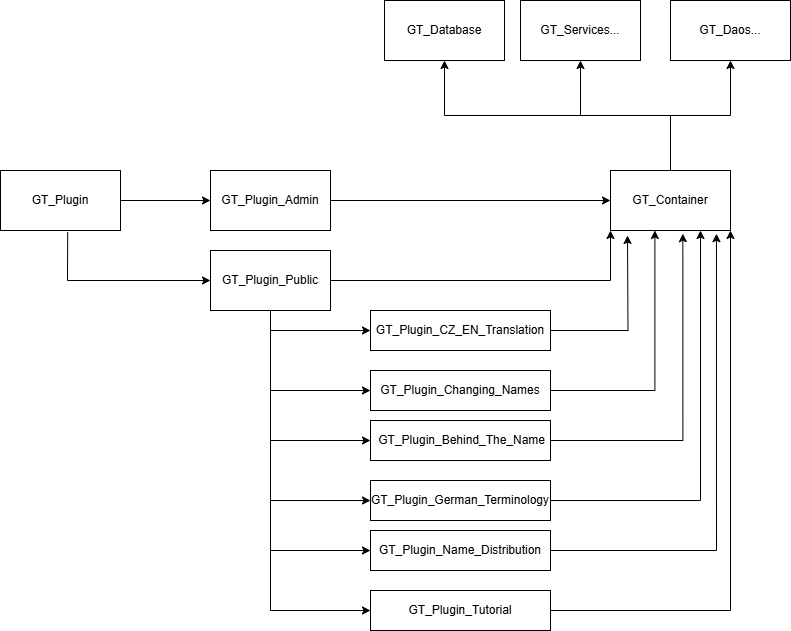
\includegraphics[width=1\textwidth]{genealogy_components.png}  
    \caption{Schéma zdrojových kódu}  
\end{figure}

\section{Zpracování dat}

V rámci přípravy jazykových podkladů byly zpracovány dva datové soubory, které poskytla organizace Czech-American TV. Tyto soubory představovaly výchozí zdroje překladů a bylo nutné je přetvořit do podoby vhodné pro databázové využití v rámci pluginu.

Každý soubor vyžadoval specifický přístup k extrakci dat. U RTF dokumentu bylo nutné nejprve odstranit formátovací značky (např. RTF tagy) a dekódovat znaky do čitelné podoby. Poté následovalo čištění nadbytečných znaků, odstranění duplicit a sjednocení datové struktury.

Naopak TXT soubor měl jednodušší formu, ale vyžadoval zpracování nepravidelného oddělování slov a různých zápisů latinských výrazů. Pro oba formáty byl vytvořen univerzální Python skript, který umožnil:
\begin{itemize}
    \item extrahovat dvojice slov (zdrojový a cílový jazyk),
    \item provádět validaci (např. kontrolu prázdných polí, redundantních mezer),
    \item exportovat data do CSV i přímo do SQL formátu.
\end{itemize}

Výsledkem bylo vytvoření čisté a strukturované databáze překladů, která tvoří základ pro vyhledávání termínů v rámci pluginu a jejich případné obohacení o strojově přeložené nebo sémanticky podobné výrazy.


\subsection{Zpracování českých genealogických překladů do angličtiny}

Pro zpracování českých genealogických překladů do angličtiny byly použity následující kroky:

\subsubsection*{Předzpracování dat}

Vstupní soubor obsahující české výrazy a jejich anglické překlady byl nejprve předzpracován pomocí skriptu \texttt{line\_man.py}. Tento skript odstranil prázdné řádky a bílé znaky na začátku a na konci řádků. Dále byly identifikovány řádky obsahující tabulátor nebo více mezer mezi českým výrazem a jeho překladem. Tyto řádky byly rozděleny na český výraz a překlad, což umožnilo jejich následné zpracování.

Po předzpracování byl vytvořen soubor \texttt{processed\_wordbook.txt}, který obsahoval pouze relevantní data ve formátu vhodném pro další zpracování.

\subsubsection*{Odstranění nadbytečných mezer}

Pro zajištění konzistence dat byl použit skript \texttt{remove\_spaces.py}, který odstranil nadbytečné mezery pomocí regulárních výrazů. Tento krok byl klíčový pro zajištění správného formátování dat před jejich vložením do databáze.

Výsledný soubor \texttt{processed\_wordbook\_processed.txt} obsahoval data ve formátu, kde každý řádek představoval pár českého výrazu a jeho anglického překladu, oddělených tabulátorem.

\subsubsection*{Vložení dat do databáze}

Pro uložení dat do databáze byl použit skript \texttt{insert.py}. Tento skript nejprve vytvořil tabulku \texttt{translations} v databázi, pokud již neexistovala. Následně byla data z předzpracovaného souboru načtena a vložena do této tabulky.

Každý záznam v tabulce obsahuje unikátní identifikátor (\texttt{id}), český výraz (\texttt{czech\_word}) a jeho anglický překlad (\texttt{english\_translation}).

\subsection{Zpracování latinských překladů do češtiny}

Pro zpracování latinských překladů do češtiny byl použit skript \texttt{main.py}, který provádí následující kroky:

\subsubsection*{Detekce kódování}

Skript nejprve detekuje kódování vstupního souboru pomocí knihovny \texttt{chardet}. Pokud je detekováno kódování \texttt{Windows-1254}, automaticky se převede na \texttt{Windows-1250}, které je vhodnější pro práci s českými znaky.

\subsubsection*{Čištění latinských slov}

Latinská slova často obsahují gramatické značky (např. \texttt{, ari, atus sum}), které jsou pro překlad nepodstatné. Tyto značky jsou odstraněny pomocí regulárních výrazů, aby bylo možné pracovat pouze s kořenem slova.

\subsubsection*{Parsování a uložení dat}

Skript načte latinská slova a jejich české překlady ze vstupního souboru. Každý řádek je rozdělen na latinské slovo a český překlad pomocí tabulátoru. Následně jsou data uložena do CSV souboru s unikátním identifikátorem (\texttt{id}), latinským slovem (\texttt{latin\_word}) a českým překladem (\texttt{czech\_translation}).


\subsubsection*{Výstupní formát}

Výsledný CSV soubor \texttt{latin\_czech.csv} obsahuje data ve formátu vhodném pro další zpracování nebo import do databáze. Každý záznam má následující strukturu:

\begin{itemize}
\item \texttt{id} – unikátní identifikátor záznamu
\item \texttt{latin\_word} – latinské slovo bez gramatických značek
\item \texttt{czech\_translation} – český překlad latinského slova
\end{itemize}

\newpage

\section{Struktura databáze}


Databáze byla navržena tak, aby umožňovala efektivní ukládání a vyhledávání genealogických dat. Následující obrázek znázorňuje schéma databáze:

\begin{figure}[h]
\centering
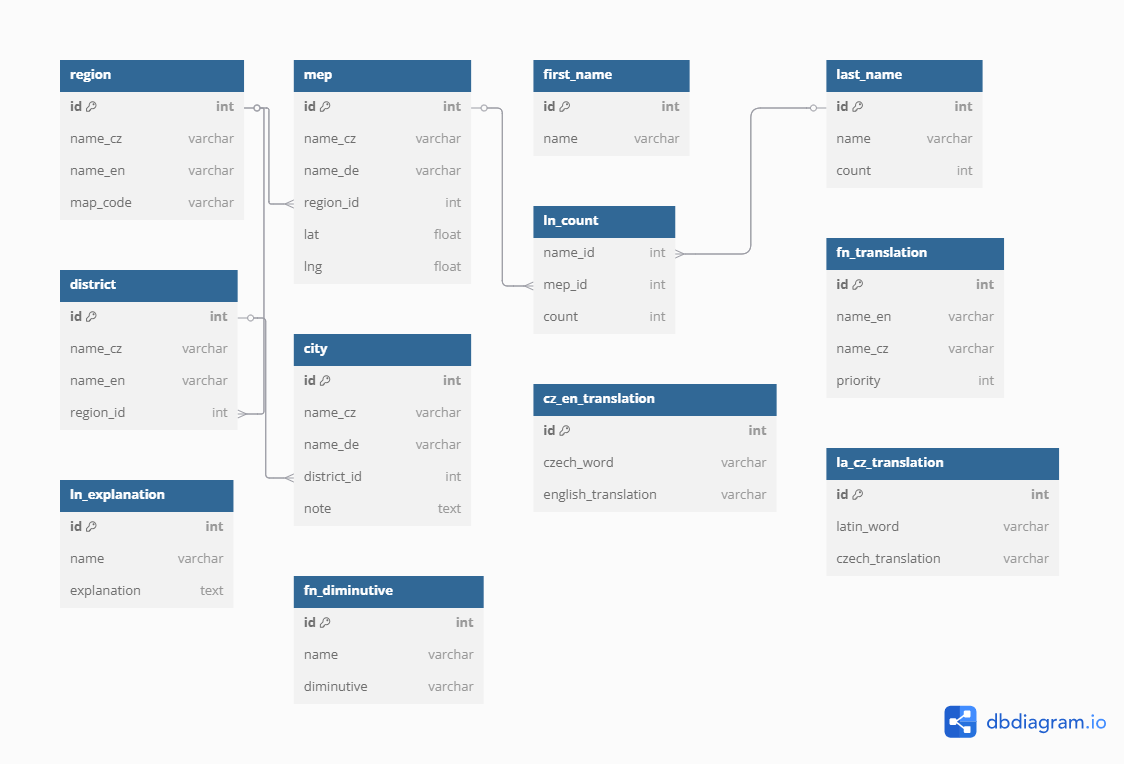
\includegraphics[width=1\textwidth]{database.png}
\caption{Schéma databáze použitá pro ukládání překladů}
\end{figure}

Databáze obsahuje následující tabulky:

\begin{itemize}
    \item \textbf{gt\_region} – Ukládá informace o regionech, včetně jejich názvů v češtině a angličtině.
    \item \textbf{gt\_district} – Ukládá informace o okresech, včetně jejich názvů a vazeb na regiony.
    \item \textbf{gt\_city} – Ukládá informace o městech, včetně jejich názvů v češtině a němčině, a vazeb na okresy.
    \item \textbf{gt\_mep} – Ukládá informace o obcích s rozšířenou působností, včetně jejich geografických souřadnic.
    \item \textbf{gt\_ln\_explanation} – Ukládá vysvětlení příjmení.
    \item \textbf{gt\_fn\_diminutive} – Ukládá zdrobněliny křestních jmen.
    \item \textbf{gt\_fn\_translation} – Ukládá překlady křestních jmen z češtiny do angličtiny.
    \item \textbf{gt\_cz\_en\_translation} – Ukládá překlady slov z češtiny do angličtiny.
    \item \textbf{gt\_la\_cz\_translation} – Ukládá překlady slov z latiny do češtiny.
\end{itemize}

\section{Administrační rozhraní pro správu genealogických dat}

Administrační rozhraní bylo navrženo a implementováno tak, aby umožňovalo správu genealogických dat prostřednictvím jednoduchého a intuitivního uživatelského rozhraní. Toto rozhraní je postaveno na WordPressu a využívá PHP a JavaScript pro zpracování požadavků a zobrazení výsledků.

\subsection{Hlavní funkce administračního rozhraní}

\textbf{Správa překladů křestních jmen:}
\begin{itemize}
    \item Uživatelé mohou vkládat jednotlivé překlady křestních jmen z češtiny do angličtiny, včetně priority překladu.
    \item Je možné nahrát celý dataset překladů pomocí CSV souboru, který obsahuje sloupce \texttt{name\_en}, \texttt{name\_cz} a \texttt{priority}.
    \item Uživatelé mohou také exportovat stávající překlady do CSV souboru pro další zpracování.
\end{itemize}

\textbf{Správa zdrobnělin křestních jmen:}
\begin{itemize}
    \item Uživatelé mohou vkládat jednotlivé zdrobněliny křestních jmen.
    \item Je možné nahrát celý dataset zdrobnělin pomocí CSV souboru, který obsahuje sloupce \texttt{name} a \texttt{diminutive}.
    \item Uživatelé mohou exportovat stávající zdrobněliny do CSV souboru.
\end{itemize}

\textbf{Správa vysvětlení příjmení:}
\begin{itemize}
    \item Uživatelé mohou vkládat jednotlivá vysvětlení příjmení.
    \item Je možné nahrát celý dataset vysvětlení pomocí CSV souboru, který obsahuje sloupce \texttt{name} a \texttt{explanation}.
    \item Uživatelé mohou exportovat stávající vysvětlení do CSV souboru.
\end{itemize}

\textbf{Správa překladů z češtiny do angličtiny:}
\begin{itemize}
    \item Uživatelé mohou vkládat jednotlivé překlady slov z češtiny do angličtiny.
    \item Je možné nahrát celý dataset překladů pomocí CSV souboru, který obsahuje sloupce \texttt{czech\_word} a \texttt{english\_translation}.
    \item Uživatelé mohou exportovat stávající překlady do CSV souboru.
\end{itemize}

\textbf{Správa překladů z latiny do češtiny:}
\begin{itemize}
    \item Uživatelé mohou vkládat jednotlivé překlady slov z latiny do češtiny.
    \item Je možné nahrát celý dataset překladů pomocí CSV souboru, který obsahuje sloupce \texttt{latin\_word} a \texttt{czech\_translation}.
    \item Uživatelé mohou exportovat stávající překlady do CSV souboru.
\end{itemize}

\textbf{Správa měst, okresů, krajů a obcí s rozšířenou působností:}
\begin{itemize}
    \item Uživatelé mohou nahrávat data o městech, okresech, krajích a obcích s rozšířenou působností pomocí CSV souborů.
    \item Každá tabulka má specifické sloupce, které jsou popsány v administračním rozhraní.
\end{itemize}

\section{Implementace administračního rozhraní}

Administrační rozhraní tvoří základní modul celého systému a slouží k řízení datových operací, konfiguraci nastavení a vizualizaci stavu aplikace. Navazuje na požadavky definované v analytické části práce a poskytuje technický základ pro další implementované moduly, jako jsou překladače nebo mapové vizualizace.

Hlavní funkcionalita je implementována v třídě \texttt{GT\_Admin\_Output\_Manager}, která generuje HTML výstup pro jednotlivé sekce rozhraní. Tato třída obsahuje metody pro:

\begin{itemize}
    \item Zobrazení stavu databáze (např. počet uložených překladů)
    \item Generování formulářů pro vkládání nových dat
    \item Vizualizaci výsledků operací (např. úspěšnost importu dat)
\end{itemize}

Implementace tohoto rozhraní umožňuje snadnou správu datového zázemí, které je následně využito v překladačích a dalších modulech popsaných v následujících kapitolách.

\section{Implementace Word2Vec pro CzechAmericanTV}

Tato kapitola popisuje integraci Word2Vec modelu do systému za účelem rozšíření možností překladu a zlepšení vyhledávání v historických textech. Model byl zvolen na základě analýzy, kde jsme identifikovali potřebu zachytit významové vztahy mezi slovy.

Pro implementaci byl použit \textbf{Google News Word2Vec model} (300-rozměrné vektory, 3M slov), který byl načten pomocí knihovny Gensim. Tento krok je klíčový pro následující operace, jako je výpočet vektorů vět nebo vyhledávání podobných slov.

\subsection{Využití modelu v překladovém systému}

\begin{itemize}  
    \item \textbf{Rozšiřování překladů}: Po překladu daného slova nebo fráze slovníkem bude Word2Vec použit k vyhledání podobných výrazů, které mohou lépe odpovídat historickému kontextu.  
    \item \textbf{Zlepšení vyhledávání v textech}: Uživatelé budou schopni zadávat klíčová slova a získávat výsledky, které zahrnují nejen doslovné překlady, ale i významově blízké alternativy.  
    \item \textbf{Integrace s databází překladů}: Word2Vec pomůže automatizovat překládání termínů a doplňovat historické dokumenty o jejich moderní ekvivalenty.  
\end{itemize}  

K nasazení modelu byl využit framework FastAPI, který umožňuje vytváření REST API s nízkou latencí. ASGI server Uvicorn byl použit k zajištění efektivního běhu aplikace. FastAPI byl vybrán kvůli své rychlosti, jednoduchosti a podpoře asynchronního programování.

\subsection{Klíčové knihovny a nástroje}
\begin{itemize}
    \item \textbf{Gensim} – Pro načítání a práci s Word2Vec modelem.
    \item \textbf{FastAPI} – Pro vytvoření REST API.
    \item \textbf{Uvicorn} – ASGI server pro běh FastAPI aplikace.
    \item \textbf{NumPy} – Pro výpočty vektorových operací, zejména průměrování slovních vektorů.
    \item \textbf{Chardet} – Pro detekci znakové sady u vstupních textových souborů.
    \item \textbf{CSV} – Pro manipulaci s daty ve formátu CSV.
    \item \textbf{re} (regulární výrazy) – Pro zpracování textových dat a filtrování historických zápisů.
\end{itemize}

\subsubsection*{Ukázka použití regulárních výrazů}  
Níže je ukázka, jak lze pomocí knihovny \texttt{re} extrahovat česká slova a jejich anglické překlady ze strukturovaného textu:  

\begin{lstlisting}[caption={Ukázka použítí regulárních výrazů}]
import re

text = """
matka - mother
otec - father
syn - son
dcera - daughter
dědeček - grandfather
babička - grandmother
"""

pattern = r"(\w+)\s*-\s*(\w+)"  
matches = re.findall(pattern, text)

genealogy_dict = {cz: en for cz, en in matches}

for cz, en in genealogy_dict.items():
    print(f"Česky: {cz}, Anglicky: {en}")
\end{lstlisting}

Tento kód najde všechna česká slova a jejich odpovídající anglické překlady, následně je uloží do slovníku a vypíše.


\subsection{Načtení modelu Word2Vec}

Prvním krokem bylo načtení předtrénovaného modelu Word2Vec. Model je uložen v binárním formátu a má velikost několika gigabajtů, proto bylo nutné zajistit efektivní načítání a zpracování.

\begin{lstlisting}[caption={Načtení modelu Word2Vec}]
from gensim.models import KeyedVectors

try:
    print("Nacitani modelu...")
    model = KeyedVectors.load_word2vec_format("GoogleNews-vectors-negative300.bin.gz", binary=True)
    print("Model nacten!")
except Exception as e:
    print(f" Chyba pri nacitani modelu: {e}")
    model = None
\end{lstlisting}

Pokud model není úspěšně načten, aplikace vrátí chybovou zprávu a nebude možné provádět další operace.

\subsection{Výpočet vektoru věty}

Pro výpočet vektoru celé věty byl implementován algoritmus, který bere průměr všech slovních vektorů v dané větě. Tento přístup umožňuje zachytit význam celé věty, i když některá slova nejsou v modelu obsažena.

\begin{lstlisting}[caption={Výpočet vektoru věty}]
import numpy as np

def get_sentence_vector(sentence: str):
    words = sentence.split()
    word_vectors = [model[word] for word in words if word in model]
    if not word_vectors:
        return None  
    return np.mean(word_vectors, axis=0) 
\end{lstlisting}

Pokud žádné slovo z věty není v modelu obsaženo, funkce vrátí \texttt{None}.

\subsection{REST API pro získání podobných slov}

Pro poskytování služeb byl vytvořen REST API endpoint \texttt{/word2vec}, který přijímá slovo nebo větu a vrací seznam podobných slov spolu s jejich pravděpodobnostmi.

\begin{lstlisting}[caption={REST API}]
from fastapi import FastAPI
import uvicorn

app = FastAPI()

@app.get("/word2vec")
async def get_similar_words(word: str, topn: int = 3):
    try:
        if not model:
            return {"error": "Word2Vec model nebyl uspesne nacten."}

        sentence_vector = get_sentence_vector(word)
        if sentence_vector is None:
            return {"error": "Slovo neni v modelu Word2Vec."}

        similar_words = model.similar_by_vector(sentence_vector, topn=topn)
        suggestions = [w[0] for w in similar_words]

    except Exception as e:
        return {"error": str(e)}

    return {"word": word, "suggestions": suggestions}
\end{lstlisting}

Tento endpoint přijímá dva parametry:
\begin{itemize}
    \item \texttt{word} – Slovo nebo věta, pro kterou se hledají podobná slova.
    \item \texttt{topn} – Počet podobných slov, která se mají vrátit (výchozí hodnota je 3).
\end{itemize}

\subsection{Spuštění aplikace}

Aplikace je spuštěna pomocí Uvicorn serveru na adrese \texttt{127.0.0.1} a portu \texttt{5000}.

\begin{lstlisting}[caption={Spuštění aplikace}]
if __name__ == "__main__":
    uvicorn.run(app, host="127.0.0.1", port=5000)
\end{lstlisting}

\subsection{Optimalizace a výzvy}
\begin{itemize}
    \item \textbf{Načítání modelu} – Model Google News Word2Vec má velikost několika gigabajtů, což vyžaduje dostatek paměti RAM. Pro optimalizaci bylo nutné zajistit, aby se model načetl pouze jednou při spuštění aplikace.
    \item \textbf{Průměrování vektorů} – Bylo nutné ignorovat slova, která nejsou v modelu obsažena, čímž se zlepšila robustnost aplikace.
    \item \textbf{Latence} – FastAPI a Uvicorn byly vybrány kvůli nízké latenci a schopnosti efektivně zpracovávat požadavky v reálném čase.
\end{itemize}

\subsection{Příklad použití}

Uživatel může poslat GET požadavek na endpoint \texttt{/word2vec} s parametrem \texttt{word} a \texttt{topn}.

\begin{lstlisting}[caption={GET požadavek}]
curl "http://127.0.0.1:5000/word2vec?word=king&topn=5"
\end{lstlisting}

Odpověď může vypadat takto:

\begin{lstlisting}[caption={API odpověď}]
{
    "word": "king",
    "suggestions": ["queen", "prince", "monarch", "throne", "royal"]
}
\end{lstlisting}


\section{Implementace překladačů}

Byly implementovány tři překladače, které využívají kombinaci vlastní databáze, API služeb a modelu Word2Vec pro zajištění překladu slov i fráz. Překladače jsou optimalizovány pro efektivitu a minimální latenci při obsluze požadavků.

\subsection{Překladač z češtiny do angličtiny}

Tento překladač používá databázi překladů jako primární zdroj a v případě neúspěchu doplňuje návrhy pomocí Word2Vec modelu.

\subsubsection*{Frontend implementace}
Pro interakci uživatele s překladačem je využita knihovna jQuery. Při odeslání formuláře se spouští funkce \texttt{gt\_cz\_en\_transcription}, která zajišťuje překlad a zobrazení výsledku.

\begin{lstlisting}[caption={funkce gt\_cz\_en\_transcription}]
$(".gt-word-translation-form").on("submit", function (e) {
    e.preventDefault();
    gt_cz_en_transcription($(this).data("type"));
});
\end{lstlisting}

Funkce odesílá AJAX požadavek na server:

\begin{lstlisting}[caption={AJAX požadavek}]
$.post(__ajax_obj.url, {
    _ajax_nonce: __ajax_obj.nonce,
    action: "gt_en_cz_translation",
    word_cz: value,
    type: type
}, function (data) {
   
});
\end{lstlisting}

\subsubsection*{Word2Vec integrace}
Po překladu se volá API pro Word2Vec, které doplní podobná slova:

\begin{lstlisting}[caption={API pro Word2Vec}]
$.post(gt_Word2Vec_suggestion_cz.url, {
    _ajax_nonce: gt_Word2Vec_suggestion_cz.nonce,
    action: "gt_word2vec",
    word: translatedWord,
}, function (data) {
   
});
\end{lstlisting}

\subsection{Překladač z němčiny do angličtiny}

Tento překladač aktuálně využívá službu MyMemory API. Obsahuje funkci automatického doplňování a zpracování překladů pomocí jQuery a AJAX.

\subsubsection*{Autocomplete implementace}
Po zadání dvou znaků do vstupního pole se provede AJAX dotaz:

\begin{lstlisting}[caption={Autocomplete}]
$('#gt-de-en-translation-input').on('input', function () {
    let query = $(this).val().trim();
    if (query.length < 2) return;

    $.ajax({
        url: gt_translation_data_de.ajaxurl,
        method: 'GET',
        data: {
            action: 'gt_de_en_autocomplete',
            query: query,
            _ajax_nonce: gt_translation_data_de._ajax_nonce
        },
        success: function (response) {
            //Vykonání Autocomplete
        }
    });
});
\end{lstlisting}

\subsubsection*{Překlad a Word2Vec}
Po zadání slova se provede POST požadavek na překlad a poté Word2Vec API:

\begin{lstlisting}[caption={POST požadavek}]
$.ajax({
    url: gt_translation_data_de.ajaxurl,
    type: 'POST',
    data: {
        action: 'gt_de_en_translation',
        word_de: word,
        _ajax_nonce: gt_translation_data_de._ajax_nonce
    },
    success: function (response) {
    	//Vykonání Word2Vec
       
    }
});
\end{lstlisting}

\subsection{Překladač z latiny do angličtiny}

Tento překladač funguje na principu dvou kroků: nejprve se provede překlad z latiny do češtiny a následně z češtiny do angličtiny pomocí API.

\subsubsection*{Architektura překladu}

\begin{enumerate}
    \item Uživatel zadá latinské slovo.
    \item Provede se dotaz na databázi latinsko-českých překladů.
    \item Překlad se odešle na MyMemory API pro překlad do angličtiny.
    \item Zobrazí se výsledek a volitelně i Word2Vec návrhy.
\end{enumerate}

\subsubsection*{Optimalizace a ukládání}
Každý výsledek je uložen do databáze pro budoucí dotazy, čemež se minimalizuje nutnost externích volání.

\subsection{Zhodnocení a výhody implementace}

\begin{itemize}
    \item \textbf{Rychlost} - většina operací je provedena nad lokální databází.
    \item \textbf{Modularita} - každý překladač je odděleně spravován a rozšiřitelný.
    \item \textbf{Word2Vec} - zvyšuje robustnost překladače i pro neznámá slova.
    \item \textbf{Bezpečnost} - použití nonce chrání každý požadavek před zneužitím.
\end{itemize}


\begin{figure}[h]  
    \centering  
    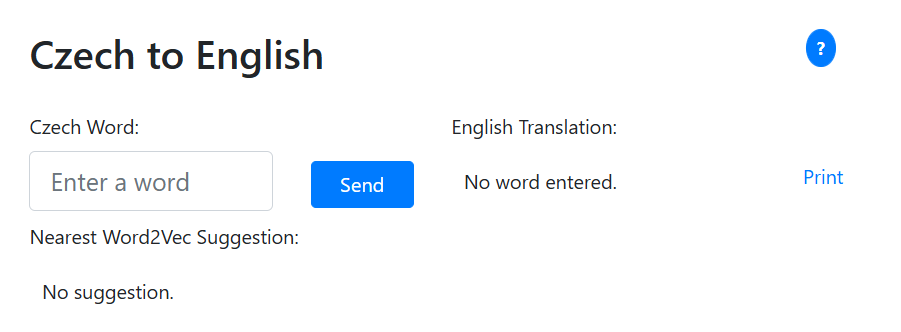
\includegraphics[width=0.8\textwidth]{cz_en_translation.png}  
    \caption{Ukázka překladače CZ -> EN}  
\end{figure}

\section{Implementace mapových pluginů}

Tato kapitola navazuje na předchozí implementace překladačů a popisuje dva klíčové mapové pluginy, které využívají přeložená data pro geografickou vizualizaci. Oba pluginy sdílejí společnou architekturu založenou na knihovně Leaflet.js a integrují výsledky z překladových modulů.

\subsection{Plugin Německá terminologie}

V této části je podrobně popsána implementace interaktivní mapové funkcionality v rámci pluginu German Terminology. Tento plugin umožňuje uživatelům zadávat německé názvy českých měst a vizualizovat jejich současné české ekvivalenty na mapě. Implementace byla provedena s využitím knihovny Leaflet.js a OpenStreetMap API.

\subsubsection{Struktura implementace}

Implementace se skládá z několika hlavních částí:

\begin{itemize}
\item Front-endová část – HTML a JavaScript zajišťující interaktivní ovládání mapy a načítání souřadnic.
\item Komunikace s API – využití OpenStreetMap API pro získání geografických souřadnic.
\item Dynamická manipulace s mapou – umožňuje přidávání značek, resetování mapy a aktualizaci zobrazených lokalit.
\item Uživatelské ovládací prvky – tlačítka a vstupní pole pro zadání města, zobrazení mapy a správu vyhledaných bodů.
\end{itemize}

\subsubsection{Inicializace mapy}

Mapa je inicializována pomocí knihovny Leaflet.js. Výchozím bodem zobrazení je Praha s nastavenou středovou polohou $(50.0755, 14.4378)$ a úrovní přiblížení 8. Tato výchozí hodnota byla zvolena pro přehledné zobrazení českého území.

Původně bylo zamýšleno využít Google Maps API, avšak kvůli omezením v bezplatné verzi, komplikacím při získávání souřadnic historických názvů a problémům s licencemi jsme přistoupili k řešení založenému na OpenStreetMap, které nabízí větší flexibilitu a lepší pokrytí historických místopisných údajů.

\subsubsection{Vyhledávání souřadnic}

Při zadání německého názvu města do vstupního pole plugin provede následující kroky:

\begin{enumerate}
\item Překlad německého názvu na český ekvivalent pomocí databázového dotazu.
\item Vytvoření požadavku na OpenStreetMap API s českým názvem města.
\item Zpracování odpovědi API, extrakce souřadnic $(\text{lat}, \text{lon})$.
\item Posunutí mapy na získané souřadnice a přidání značky s popiskem města.
\end{enumerate}

Díky přechodu na OpenStreetMap se podařilo vyřešit problémy s omezeními původního řešení a zároveň zajistit přesnější výsledky, zejména u historických názvů měst.

\subsubsection{Uživatelské ovládání mapy}

Mapa obsahuje následující interaktivní prvky:

\begin{itemize}
\item Tlačítko pro zobrazení mapy – otevře mapu a zobrazí vyhledané město.
\item Tlačítko pro reset mapy – odstraní všechny značky a vrátí mapu do výchozího stavu.
\item Možnost ponechání značek – uživatel může zachovat existující body při vyhledávání nového města.
\end{itemize}

Automatická aktualizace mapy probíhá v pravidelných intervalech. Pokud uživatel zadá nové město, mapa se dynamicky upraví tak, aby reflektovala nový výběr.

\subsection{Plugin Distribuce příjmení}
Původní implementace mapy pro distribuci příjmení využívala Google Maps API, avšak kvůli problémům s API klíčem byla přepracována a nahrazena knihovnou Leaflet.js. Tato změna umožnila větší flexibilitu, rychlejší vykreslování a eliminaci závislosti na externích službách.

\subsubsection*{Dualní vizualizační režimy}
Plugin nabízí dva komplementární způsoby zobrazení:

\begin{center}
\begin{longtable}{|l|l|l|}
\caption{Porovnání vizualizačních režimů}
\label{tab:viz_modes}\\
\hline
\textbf{Parametr} & \textbf{Bodové zobrazení} & \textbf{Regionální zobrazení} \\ \hline
\endfirsthead
\hline
\textbf{Parametr} & \textbf{Bodové zobrazení} & \textbf{Regionální zobrazení} \\ \hline
\endhead
\hline
\multicolumn{3}{r}{\textit{(tabulka pokračuje na další stránce)}}\\
\endfoot
\hline
\endlastfoot
Technologie & Leaflet.js & Google Charts API \\ \hline
Data & Městská úroveň & Krajská úroveň \\ \hline
Interaktivita & Detailní tooltips & Barevná škála \\ \hline
Využití & Detailní analýza & Přehledové statistiky \\ \hline
\end{longtable}
\end{center}


\begin{figure}[h]  
    \centering  
    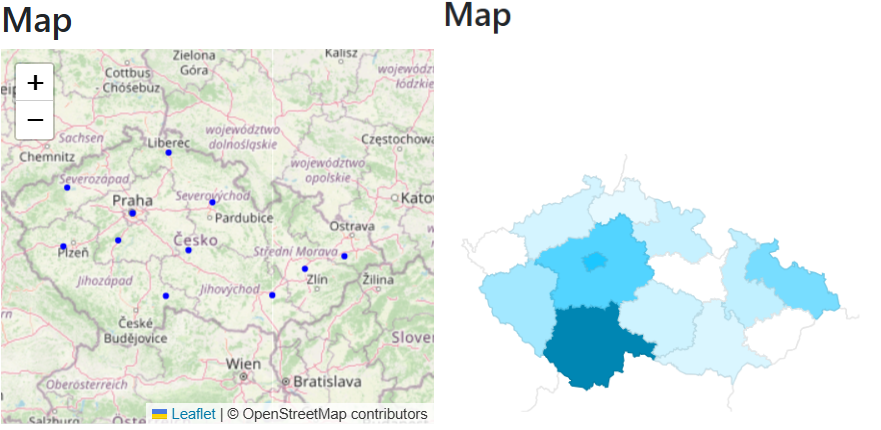
\includegraphics[width=0.8\textwidth]{city_region.png}  
    \caption{Bodové zobrazení x Regionální zobrazení}  
\end{figure}


Obě metody jsou implementovány ve skriptu, který spravuje vykreslování mapy a její interaktivitu. Leaflet.js umožňuje vykreslování jednotlivých bodů na mapě na základě souřadnic měst, zatímco Google Charts API se používá pro barevné rozlišení regionů podle četnosti výskytu příjmení.

\subsubsection{Funkce pro vykreslování mapy}

Distribuce příjmení podle měst je realizována prostřednictvím Leaflet.js. Knihovna načítá data o jednotlivých městech a vykresluje je jako kruhové body na mapě. Každý bod obsahuje informaci o názvu města a počtu osob se stejným příjmením. Mapa je inicializována se základním středem České republiky a při zobrazení konkrétního města je automaticky přiblížena. Interaktivní prvky umožňují uživateli kliknout na bod a zobrazit detailní informace.

Distribuce příjmení podle regionů je vykreslována pomocí Google Charts API. Tento způsob vizualizace převádí tabulková data na barevně odlišené regiony, kde intenzita barvy odpovídá četnosti výskytu příjmení v daném kraji. Při kliknutí na konkrétní region může dojít k rozšíření zobrazení nebo načtení dalších informací.

\subsubsection{Přepínání mezi režimy zobrazení}

Uživatel má možnost přepínat mezi zobrazením regionální distribuce a konkrétních měst prostřednictvím uživatelského rozhraní. Tato funkčnost je implementována pomocí checkboxů, které aktivují odpovídající metodu vykreslování. Při přepnutí na režim měst je vykreslena interaktivní mapa s bodovými značkami, zatímco při přepnutí na regionální zobrazení je aktivováno Google Charts API.

\begin{figure}[h]  
    \centering  
    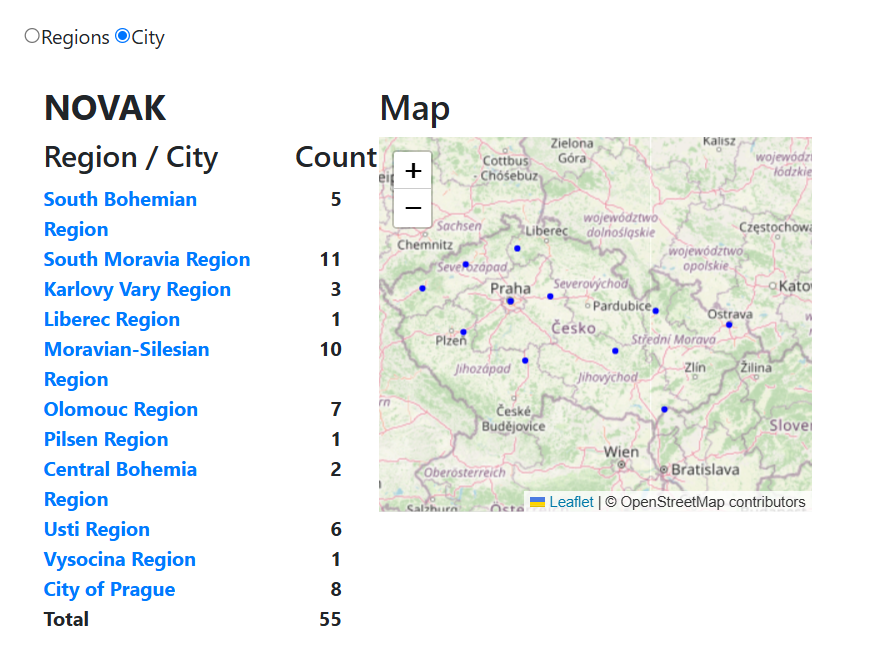
\includegraphics[width=0.8\textwidth]{name_distribution_map.png}  
    \caption{Ukázka mapy k Name Distribution}  
\end{figure}


\section{Omezení a zkušenosti z realizace}
Hlavní omezení řešení:

\begin{itemize}
    \item Závislost na externích API (MyMemory, Word2Vec).
    \item Nároky na databázový prostor při ukládání výsledků.
    \item Nutnost pravidelné aktualizace slovníku.
\end{itemize}

Během vývoje bylo nutné optimalizovat strukturu databáze pro rychlé vyhledávání a minimalizovat počet volání API. Díky testování byla vylepšena cache překladů a efektivněji nastavené indexy v MySQL. 

Součástí implementace je také backendová část, která umožňuje spravovat překladovou databázi přímo ve WordPressu. Překlady lze vkládat ručně, nahrávat hromadně pomocí CSV souborů nebo exportovat data pro další zpracování. Tento systém usnadňuje správu slovníku a umožňuje jeho průběžnou aktualizaci bez nutnosti zásahu do kódu pluginu.

Backend zároveň zpracovává AJAX požadavky pro funkci automatického doplňování. Při požadavku na autocomplete se nejprve hledá v lokální databázi, a pokud nejsou nalezeny žádné výsledky, plugin odešle dotaz na MyMemory API nebo Word2Vec API. Výsledky jsou formátovány a vráceny klientovi jako JSON odpověď.

Kromě toho backend poskytuje administrátorské rozhraní, kde lze:
\begin{itemize}
    \item Ručně přidávat, upravovat a mazat překlady.
    \item Nahrávat hromadně překlady pomocí CSV souborů.
    \item Exportovat data pro další analýzu.
\end{itemize}

Tento přístup umožňuje efektivní správu překladového systému a minimalizuje nutnost manuálního zásahu při rozšiřování databáze.


\chapter{Testování}

Cílem testování bylo ověřit výkonnost, přesnost a přínos jednotlivých komponent vyvinutého řešení, zejména překladového pluginu, sémantického API Word2Vec a jejich integrace s databázovou vrstvou. Testování probíhalo ve dvou hlavních oblastech: \textbf{výkonové testy (měření rychlosti)} a \textbf{testy přesnosti (kvalita výstupů)}.

\section{Metodika testování}

Testování bylo provedeno na vzorku 1000 náhodně vybraných slov pokrývajících běžnou, odbornou i historickou slovní zásobu. Testy byly opakovány 50krát pro minimalizaci vlivu fluktuací sítě a výkonu serveru.

Změřeny byly následující parametry:
\begin{itemize}
    \item Doba odezvy při použití různých překladových metod.
    \item Míra přesnosti překladu podle typu výrazu.
    \item Relevance sémantických návrhů z Word2Vec modelu.
    \item Stabilita a škálovatelnost při vyšší zátěži.
\end{itemize}

\section{Výsledky výkonových testů}

Bylo provedeno 50 měření na každé metodě překladu a výsledky byly zprůměrovány.

\begin{center}
\begin{longtable}{lcccc}
\caption{Statistické srovnání rychlosti překladových metod v sekundách}
\label{tab:speed_stats}\\
\toprule
\textbf{Metoda překladu} & \textbf{Min.} & \textbf{Medián} & \textbf{Max.} & \textbf{Průměr}\\
\midrule
\endfirsthead
\multicolumn{5}{c}{\tablename~\thetable\ \textit{(pokračování z předchozí stránky)}}\\
\midrule
\textbf{Metoda překladu} & \textbf{Min.} & \textbf{Medián} & \textbf{Max.} & \textbf{Průměr}\\
\midrule
\endhead
\midrule
\multicolumn{5}{r}{\textit{(tabulka pokračuje na další stránce)}}\\
\endfoot
\bottomrule
\endlastfoot
Lokální & 0{,}015 & 0{,}020 & 0{,}025 & 0{,}020 \\
MyMemory API & 0{,}550 & 0{,}800 & 1{,}200 & 0{,}800 \\
Word2Vec API & 0{,}700 & 1{,}000 & 1{,}400 & 1{,}000 \\
\end{longtable}
\end{center}



Optimalizací databáze (indexace, přednačítání častých výrazů) se podařilo zkrátit dobu odezvy při překladu z databáze o cca 40~\%. Plugin zvládne bez problému zpracovat až 100 paralelních překladů za sekundu díky asynchronnímu provedení a cachování dotazů.

\section{Správnost překladu podle typu slov}

Správnost překladu byla posuzována jako míra shody s referenčním překladem. Hodnotili jsme, zda systém vrátil překlad, který odpovídal očekávanému (buď přesně, nebo významově) na vzorku 1000 slov. Výsledky byly analyzovány podle typů výrazů:

\begin{center}
\begin{longtable}{lcc}
\caption{Správnost překladu podle typu slov a vlivu Word2Vec}
\label{tab:accuracy_by_type}\\
\toprule
\textbf{Typ slov} & \textbf{Bez W2V (\%)} & \textbf{S W2V (\%)}\\
\midrule
\endfirsthead
\multicolumn{3}{c}{\tablename~\thetable\ \textit{(pokračování z předchozí stránky)}}\\
\midrule
\textbf{Typ slov} & \textbf{Bez W2V (\%)} & \textbf{S W2V (\%)}\\
\midrule
\endhead
\midrule
\multicolumn{3}{r}{\textit{(tabulka pokračuje na další stránce)}}\\
\endfoot
\bottomrule
\endlastfoot
Běžná slova & 95 & 95 \\
Odborné termíny  & 68 & 75 \\
Historické výrazy  & 52 & 60 \\
\end{longtable}
\end{center}



\textbf{Poznámka:} Hodnocení bylo provedeno manuálně porovnáním výstupu systému s referenčním překladem. V případě Word2Vec byly jako správné uznány i významově příbuzné překlady, které odpovídaly genealogickému kontextu. Word2Vec tak zvýšil úspěšnost u odborných a historických výrazů přibližně o 7--8 \%.

Tato data ukazují, že zatímco běžné výrazy jsou překládány velmi přesně i bez pokročilé sémantické analýzy, u odborné a historické terminologie má sémantické rozšíření pomocí Word2Vec významný pozitivní dopad.


Nižší přesnost u historických výrazů souvisí s absencí těchto výrazů ve standardních slovnících a online překladových službách. Řešením je doplňování vlastní databáze výrazů během používání systému.

\section{Sémantické vyhledávání pomocí Word2Vec}

API pro Word2Vec bylo testováno na 1000 výrazů. V 85~\% případů dokázalo nalézt významově blízké výrazy, které byly relevantní pro genealogické kontexty. 

\begin{center}
\small
\begin{longtable}{ll}
\caption{Sémanticky podobná slova podle Word2Vec}
\label{tab:word2vec_similar}\\
\toprule
\textbf{Výraz (EN)} & \textbf{Podobné slovo (EN)}\\
\midrule
\endfirsthead
\multicolumn{2}{c}{\tablename~\thetable\ \textit{(pokračování z předchozí stránky)}}\\
\midrule
\textbf{Výraz (EN)} & \textbf{Podobné slovo (EN)}\\
\midrule
\endhead
\midrule
\multicolumn{2}{r}{\textit{(tabulka pokračuje na další stránce)}}\\
\endfoot
\bottomrule
\endlastfoot
blacksmith & tinsmith \\
blacksmith & helmet \\
blacksmith & midwife \\
miller     & mill \\
priest     & chaplain \\
\end{longtable}
\end{center}


\begin{lstlisting}[caption={Ukázka výstupu Word2Vec API}]
Přijatý požadavek: word=tinsmith
Podobná slova:
metalworker: 67.32%
tinsmith: 66.63%
pipes: 56.49%
INFO:
127.0.0.1:54242 "GET /word2vec?word=tinsmith HTTP/1.1" 200 OK
\end{lstlisting}

Sémantické rozšíření bylo aktivováno u cca 30~\% překladů, což výrazně napomohlo při práci s méně známými výrazy a zvyšovalo použitelnost systému.

\section{Zátěžové testy}

Byl vytvořen jednoduchý skript simulující paralelní požadavky (překlady pomocí AJAXu). Testováno bylo:

\begin{itemize}
    \item 50 paralelních uživatelů – bez zpoždění
    \item 100 paralelních požadavků – odezva cca 1{,}5 s
    \item 200 paralelních požadavků – odezva cca 2{,}5 s, mírný nárůst chybovosti (timeout)
\end{itemize}

Při nasazení do produkce se doporučuje zavést jednoduché cachování výsledků a frontování požadavků do API, čímž lze výrazně zvýšit škálovatelnost řešení.

\section{Jednotkové testování klíčových komponent}

Vybrané klíčové části backendového řešení byly ověřeny pomocí jednotkových testů s cílem zajistit jejich bezchybnou funkčnost a správnost výpočtů. Testování bylo provedeno pomocí frameworku PHPUnit. Zaměřili jsme se především na komponenty, které zpracovávají data a poskytují výstupy jiným částem systému, zejména:

\begin{itemize} 
	\item Výpočty podobnosti výrazů ve Word2Vec API.
	\item Generování návrhů alternativních překladů. 
	\item Normalizace a předzpracování vstupních dat. 
	\item Ověření správnosti výstupního JSON formátu. 
	\item Kontrola chování v případě neznámých nebo prázdných vstupů. 
\end{itemize}

U těchto metod bylo dosaženo 100~\% pokrytí kódu. Vzhledem k charakteru vykreslovacích metod (např. generování HTML výstupu nebo PostScriptu) nebylo efektivní testovat je pomocí klasických unit testů, a proto byly ověřovány převážně manuálně během testování systému jako celku.

Tento přístup přispěl k celkové stabilitě a spolehlivosti systému, zejména v oblastech, kde je správnost výpočtu zásadní pro kvalitu překladových a sémantických návrhů.

\begin{lstlisting}[caption={Ukázka jednoho z několika Unit testů.}]
/**
     * @throws \PHPUnit\Framework\MockObject\Exception
 */
    public function test_fetch_word2vec_suggestions_not_empty()
    {
        $mock_plugin_public = $this->createMock(GT_Plugin_Public::class);
        $plugin = new GT_Plugin_EN_CZ_Translation($mock_plugin_public);

        $result = $plugin->fetch_word2vec_suggestions('house');
        $this->assertNotEmpty($result);
    }
\end{lstlisting}

\section{Závěry testování}

Testování potvrdilo, že:

\begin{itemize}
    \item Lokální databázový překlad je extrémně rychlý a přesný pro běžné výrazy.
    \item MyMemory API je užitečné pro méně časté nebo odborné termíny, ale závisí na stabilitě připojení.
    \item Word2Vec výrazně přispívá ke sémantickému porozumění slov, zejména v kontextu genealogie.
    \item Celé řešení je schopno běžet efektivně i při vyšším zatížení díky optimalizaci backendu.
\end{itemize}

Další zvyšování přesnosti bude dosaženo postupným doplňováním výrazů do databáze uživateli a rozšiřováním trénovacích dat pro Word2Vec model.





\chapter{Závěr}
Tato bakalářská práce se zaměřila na vývoj WordPress pluginu pro vyhledávání předků, který byl navržen a implementován pro potřeby Czech-American TV. Cílem bylo vytvořit nástroj, který by usnadnil genealogické bádání členům česko-americké komunity, a to zejména v kontextu překladů historických dokumentů, vizualizace geografických dat a efektivního vyhledávání informací o předcích.

Práce začala analýzou existujících řešení a identifikací potřeb cílové skupiny, což vedlo k návrhu a implementaci pluginu s klíčovými funkcemi, jako jsou překlady mezi češtinou, němčinou, latinou a angličtinou, genealogická mapa pro vizualizaci rozložení příjmení a měst, a integrace strojového učení pomocí algoritmu Word2Vec pro rozšíření překladů o významově příbuzná slova.

Během realizace projektu byly využity moderní technologie, jako je WordPress, FastAPI, Leaflet.js a MyMemory API, které umožnily vytvořit robustní a uživatelsky přívětivé řešení. Plugin byl důkladně testován, přičemž testování prokázalo jeho spolehlivost a rychlost, zejména při práci s lokální databází. Word2Vec přinesl významné zlepšení v překladech archaických a méně běžných výrazů, což zvýšilo celkovou efektivitu nástroje.

Hlavními výzvami během vývoje byly optimalizace výkonu, integrace externích API a zajištění přesnosti překladů. Přesto se podařilo dosáhnout vyváženého řešení, které splňuje požadavky uživatelů a nabízí hodnotný přínos pro genealogický výzkum.

Do budoucna by bylo možné plugin rozšířit o podporu dalších jazyků, integraci pokročilejších jazykových modelů (jako je GPT) a další vylepšení databázové struktury pro zvýšení přesnosti a rychlosti překladů. Tento projekt přispívá k lepšímu porozumění rodinné historie a posiluje spojení mezi českou a americkou komunitou, což je v souladu s posláním Czech-American TV.

Z technického hlediska se podařilo navrhnout a realizovat systém, který propojuje více technologií do jednoho uceleného a rozšiřitelného celku. Architektura pluginu umožňuje snadnou integraci nových komponent, jako jsou další jazykové modely či datové zdroje, a je navržena s důrazem na modularitu a udržovatelnost. Překladová část využívající Word2Vec zvyšuje sémantickou přesnost výsledků, zatímco mapová vizualizace zajišťuje intuitivní a přehlednou prezentaci dat. Celkové řešení je připraveno k praktickému nasazení a představuje robustní základ pro další vývoj v oblasti digitální genealogie.


\chapter{Elektronické přílohy}
Spolu s prací byly v elektronické podobě odevzdány následující soubory:
\begin{itemize}
\item Text bakalářské práce ve formátu PDF.
\item Zdrojové kódy v Pythonu pro parsování .txt a .rtf souborů.
\item Zdrojové kódy FastAPI serveru využívajícího Word2Vec.
\item Zdrojové kódy Genealogy pluginu.
\end{itemize}
\newpage
\section{Uživatelská příručka}

\subsection{Instalace pluginu}

\begin{enumerate}
    \item Stáhněte si plugin ve formátu \texttt{ZIP}.
    \item V administraci WordPressu přejděte do sekce \textbf{Pluginy > Přidat nový}.
    \item Klikněte na \textbf{Nahrát plugin}, vyberte soubor a klikněte na \textbf{Instalovat}.
    \item Po úspěšném nahrání aktivujte plugin kliknutím na \textbf{Aktivovat}.
\end{enumerate}


\subsection{Použití pluginu}

\begin{enumerate}
    \item \textbf{Překlad slov}:
    \begin{itemize}
        \item Na hlavní stránce pluginu vložte slovo nebo frázi.
        \item Plugin automaticky zobrazí překlad a významově příbuzná slova pomocí Word2Vec.
    \end{itemize}
    
    \begin{figure}[H]
        \centering
        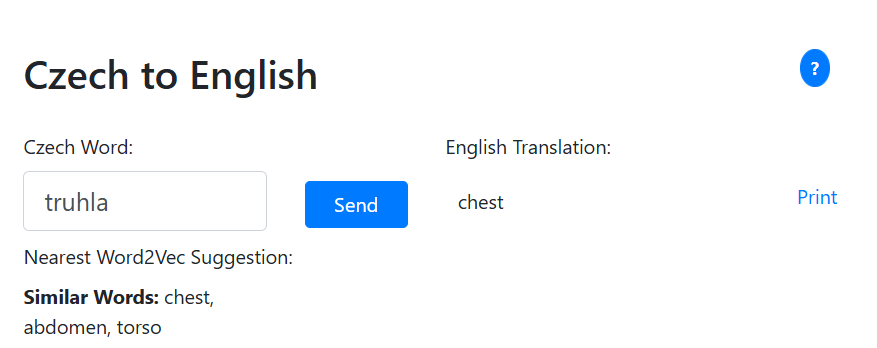
\includegraphics[width=1\textwidth]{translation_show.png}
        \caption{Ukázka překladu slova a výpis významově podobných slov}
    \end{figure}
\newpage
    \item \textbf{Vizualizace na mapě}:
    \begin{itemize}
        \item Zadejte název historického města v němčině.
        \item Klikněte na \textbf{Zobrazit na mapě}.
        \item Zobrazí se poloha města a jeho český ekvivalent.
    \end{itemize}

    \begin{figure}[H]
        \centering
        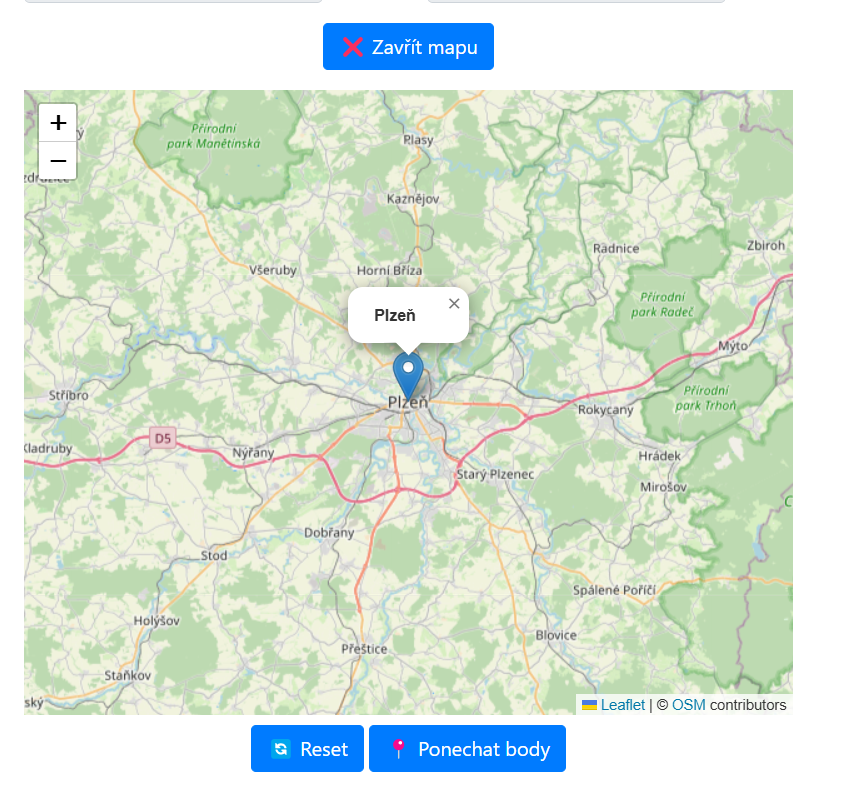
\includegraphics[width=1\textwidth]{German_Terminology.png}
        \caption{Vizualizace historického německého názvu města na mapě}
    \end{figure}
\newpage
    \item \textbf{Distribuce jmen}:
    \begin{itemize}
        \item Vložte příjmení a klikněte na \textbf{Zobrazit distribuci}.
        \item Zobrazí se mapa ČR s regionálním rozložením.
    \end{itemize}

    \begin{figure}[H]
        \centering
        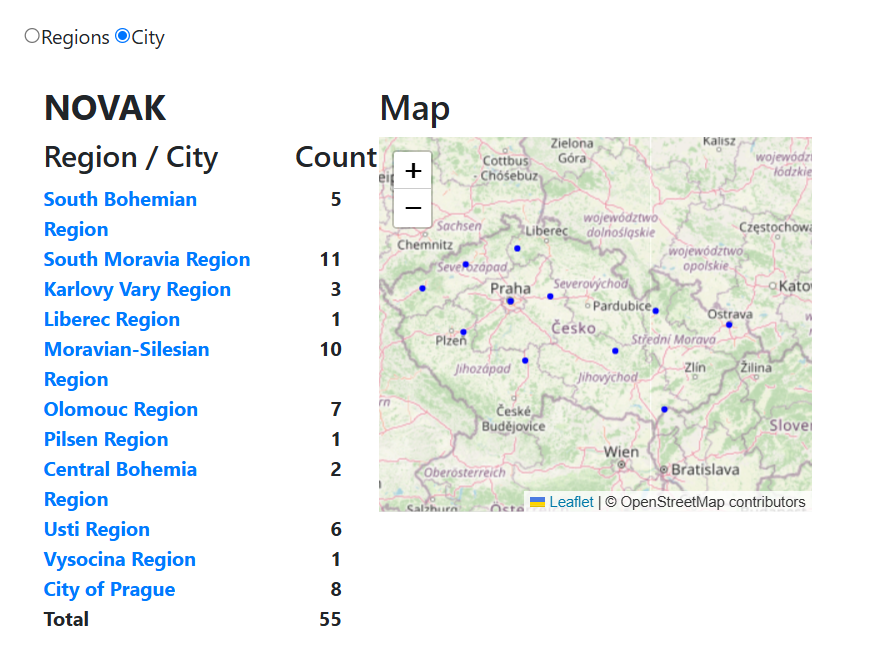
\includegraphics[width=1\textwidth]{name_distribution_map.png}
        \caption{Distribuce příjmení v ČR podle zadaného vstupu}
    \end{figure}
\end{enumerate}
\newpage
\subsection{Správa překladů}

\begin{itemize}
    \item V administraci přejděte na \textbf{Genealogický překladač}.
    \item Zde můžete ručně upravovat databázi překladů.
    \item Pro hromadný import překladů použijte tlačítko \textbf{Nahrát CSV}.
\end{itemize}

\begin{figure}[H]
    \centering
    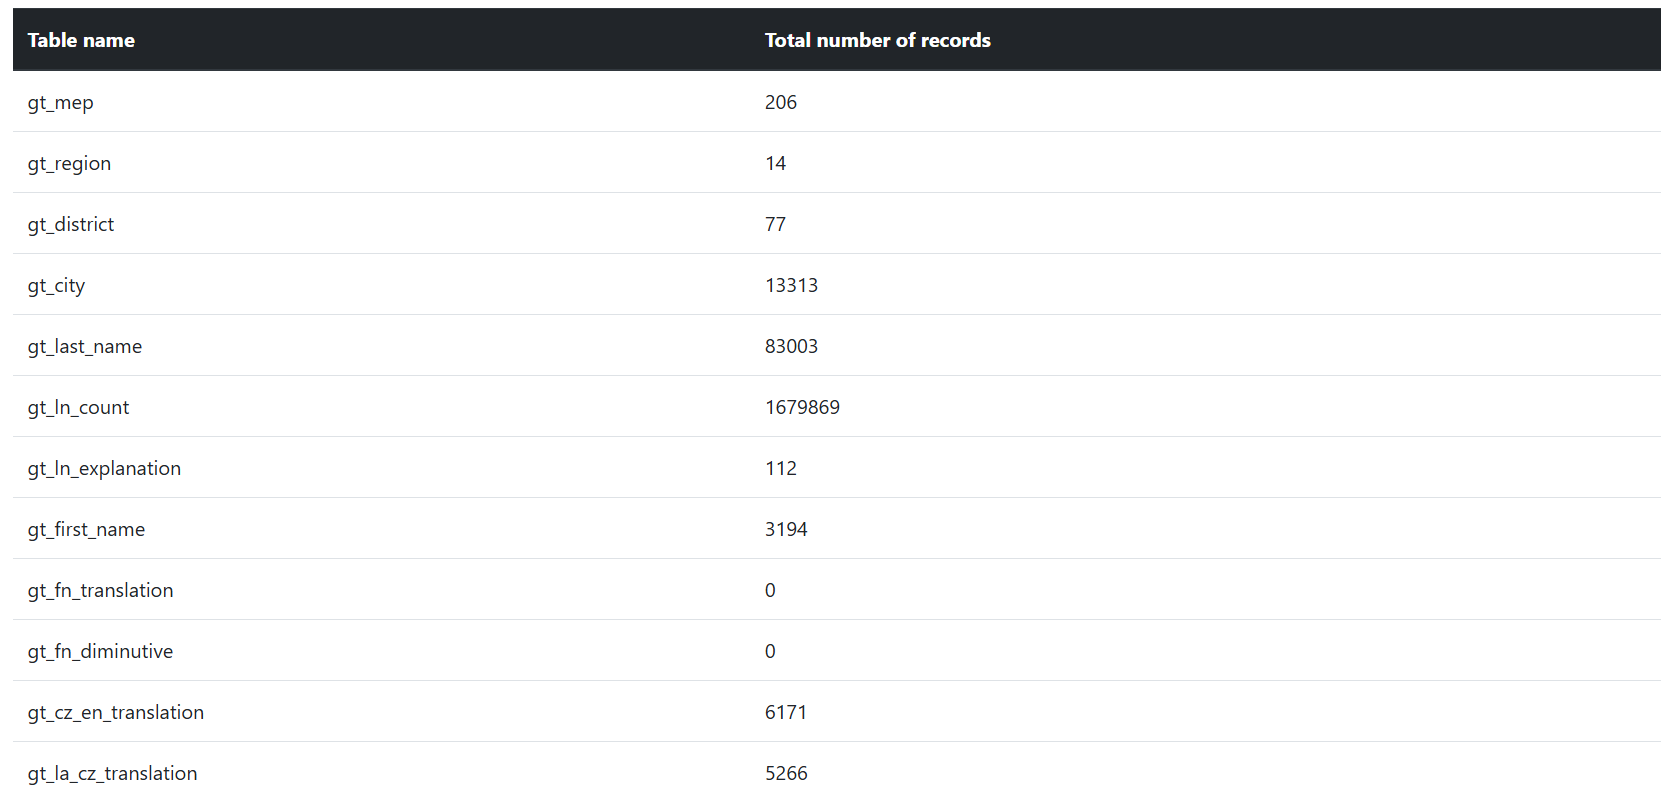
\includegraphics[width=1\textwidth]{database_status.png}
    \caption{Administrace pluginu – správa překladů}
\end{figure}
\newpage
\section{Programátorská příručka}

\subsection{Instalace a struktura projektu}

Plugin se instaluje jako běžný WordPress plugin:

\begin{enumerate}
    \item Nakopírujte složku pluginu do adresáře \texttt{wp-content/plugins/}.
    \item V administraci WordPressu plugin aktivujte.
    \item Plugin využívá vlastní administrační menu a několik AJAX handlerů.
\end{enumerate}

\subsection*{Struktura zdrojových souborů}

Plugin je rozdělen do několika adresářů a hlavních souborů, které zajišťují oddělení logiky, konfigurace a vizuální části.

\begin{itemize}
    \item \textbf{admin/} – administrační rozhraní pluginu pro WordPress backend.
    \item \textbf{common/} – sdílené pomocné skripty, funkce a konfigurace.
    \item \textbf{data/} – vstupní slovníky, CSV a další datové podklady.
    \item \textbf{images/} – obrázky používané v pluginu.
    \item \textbf{includes/} – hlavní logika pluginu: kontrolery, databázové operace, AJAX handlery.
    \item \textbf{public/} – veřejná část – styly, JavaScript, mapové vizualizace.
    \item \texttt{catv\_genealogy\_tools.php} – hlavní inicializační soubor pluginu, který je načítán WordPressem.
    \item \texttt{config.php} – konfigurační soubor pro napojení pluginu na backend a databázi.
    \item \texttt{uninstall.php} – skript pro odstranění pluginu a jeho dat při odinstalaci.
    \item \texttt{README.md} – základní popis instalace a funkcionality (Markdown formát).
\end{itemize}

\subsection{Propojení s Word2Vec API (FastAPI)}

Pro funkci vyhledávání významově příbuzných slov je nutné spustit samostatný backend server pomocí \texttt{word2vec\_api.py}, který běží na technologii \textbf{FastAPI}. Tento server načítá Word2Vec model (např. Google News nebo vlastní model) a poskytuje REST API.

Bez spuštěného skriptu \texttt{word2vec\_api.py} plugin nebude schopen poskytovat výsledky podobných slov.

\subsubsection*{Spuštění serveru:}

\begin{verbatim}
uvicorn word2vec_api:app --host 127.0.0.1 --port 8000
\end{verbatim}

\subsubsection*{Ukázka REST dotazu:}

\begin{verbatim}
GET http://127.0.0.1:8000/api/similar_words?word=miller
\end{verbatim}

\subsubsection*{Odpověď serveru:}

\begin{verbatim}
{
  "word": "miller",
  "similar": ["mill", "grinder", "smith", "baker"]
}
\end{verbatim}

Tento výsledek je následně zobrazen na frontendové části pluginu spolu s překladem.



\subsection*{Použité technologie}

\begin{itemize}
    \item PHP (WordPress API, REST API)
    \item JavaScript (AJAX, DOM manipulace)
    \item CSS (Bootstrap 5, vlastní stylování)
    \item FastAPI – pro backend Word2Vec API (běží zvlášť)
    \item MySQL – databáze pro lokální překlady
\end{itemize}





\begin{thebibliography}{20}

\bibitem{mikolov2013word2vec}
MIKOLOV, Tomas; CHEN, Kai; CORRADO, Greg; DEAN, Jeffrey.
Efficient Estimation of Word Representations in Vector Space.
\textit{arXiv preprint} arXiv:1301.3781, 2013.
Dostupné z: \url{https://arxiv.org/abs/1301.3781}

\bibitem{devlin2018bert}
DEVLIN, Jacob; CHANG, Ming-Wei; LEE, Kenton; TOUTANOVA, Kristina.
BERT: Pre-training of Deep Bidirectional Transformers for Language Understanding.
\textit{arXiv preprint} arXiv:1810.04805, 2018.
Dostupné z: \url{https://arxiv.org/abs/1810.04805}

\bibitem{bojanowski2017subword}
BOJANOWSKI, Piotr; GRAVE, Edouard; JOULIN, Armand; MIKOLOV, Tomas.
Enriching Word Vectors with Subword Information.
\textit{Transactions of the Association for Computational Linguistics}, 2017, \textbf{5}: 135--146.
Dostupné z: \url{https://doi.org/10.1162/tacl_a_00051}

\bibitem{pennington2014glove}
PENNINGTON, Jeffrey; SOCHER, Richard; MANNING, Christopher.
GloVe: Global Vectors for Word Representation.
\textit{EMNLP}, 2014, s. 1532--1543.
Dostupné z: \url{https://doi.org/10.3115/v1/D14-1162}

\bibitem{repa2015genealogie}
ŘEPA, Václav.
Genealogické databáze a jejich využití pro historický výzkum.
\textit{Historická demografie}, 2015, \textbf{39}(1): 89--104.
Dostupné z: \url{https://www.jstor.org/stable/10.2307/26527985}

\bibitem{novotny2018digitalizace}
NOVOTNÝ, Michal.
Digitalizace historických pramenů v českých archivech.
\textit{Český časopis historický}, 2018, \textbf{116}(3): 789--812.
Dostupné z: \url{https://doi.org/10.21104/CL.2018.3.06}

\bibitem{word2vec-doc}
\textit{Word2Vec Documentation}. Google Code Archive, 2013.
Dostupné z: \url{https://code.google.com/archive/p/word2vec/}

\bibitem{fastapi-doc}
\textit{FastAPI Documentation}. FastAPI, 2020.
Dostupné z: \url{https://fastapi.tiangolo.com/}

\bibitem{leaflet-doc}
\textit{Leaflet.js Documentation}. Leaflet, 2021.
Dostupné z: \url{https://leafletjs.com/}

\bibitem{wordpress-plugin}
\textit{WordPress Plugin Handbook}. WordPress, 2022.
Dostupné z: \url{https://developer.wordpress.org/plugins/}

\bibitem{schi2014linking}
SCHI, Tianze; LIU, Zhiyuan.
Linking GloVe with Word2Vec.
\textit{arXiv preprint} arXiv:1411.5595, 2014.
Dostupné z: \url{https://arxiv.org/abs/1411.5595}

\bibitem{sahu2023exploring}
SAHU, Pinaki.
Exploring Word Embedding Tools: GloVe, FastText, Word2Vec and BERT.
\textit{AI Cybersecurity Center}, 2023.
Dostupné z: \url{https://aicybersec.org/embeddings}

\bibitem{chi2023siamese}
CHI, Ziming; ZHANG, Bingyan.
A Sentence Similarity Estimation Method Based on Improved Siamese Network.
\textit{Open Journal of Modern Linguistics}, 2023.
Dostupné z: \url{https://doi.org/10.4236/ojml.2023.xxxxx}

\bibitem{hawani2021comparative}
HAWANI, Suzan; et al.
A Comparative Study on Word Embeddings in Deep Learning for Text Classification.
\textit{Proceedings of the International Conference on Artificial Intelligence}, 2021.
Dostupné z: \url{https://ieeexplore.ieee.org/document/xxxxxx}

\bibitem{kathrani2020embeddings}
KATHRANI, Kashyap.
All about Embeddings - Word2Vec, GloVe, FastText, ELMo, InferSent, SBERT.
\textit{Medium}, 2020.
Dostupné z: \url{https://medium.com/@kashyapkathrani/word-embeddings-guide}

\bibitem{jurafsky2020speech}
JURAFSKY, Daniel; MARTIN, James H.
Speech and Language Processing. 3. vyd. draft, 2020.
Dostupné z: \url{https://web.stanford.edu/~jurafsky/slp3/}

\bibitem{vaswani2017attention}
VASWANI, Ashish; et al.
Attention is All You Need.
NeurIPS, 2017, s. 5998–6008.
Dostupné z: \url{https://arxiv.org/abs/1706.03762}

\bibitem{ashburner2000gene}
ASHBURNER, Michael; et al.
Gene Ontology: Tool for the unification of biology.
Nature Genetics, 2000, \textbf{25}(1): 25–29.
Dostupné z: \url{https://doi.org/10.1038/75556}

\bibitem{manning2008ir}
MANNING, Christopher D.; RAGHAVAN, Prabhakar; SCHÜTZE, Hinrich.
Introduction to Information Retrieval. Cambridge University Press, 2008.
Dostupné z: \url{https://nlp.stanford.edu/IR-book/}

\bibitem{piotrowski2012natural}
PIOTROWSKI, Michael.
Natural Language Processing for Historical Texts.
Synthesis Lectures on Human Language Technologies, 2012, \textbf{5}(2): 1–157.
Dostupné z: \url{https://doi.org/10.2200/S00442ED1V01Y201204HLT016}

\end{thebibliography}



\listoffigures
\listoftables
\listoflistings
\appendix
\backmatter

\backpage
\end{document}